\documentclass[
  final,
  babelLanguage=portuguese,
  %desktopVersion,
  %showtrims,
  %overleaf,
]{anecdote}

\graphicspath{{./assets/photos/92dpi-ebook-sRGB/}}

% Page size: 6x9 inch
% Body text: 10.5 / 15 pt

\usepackage{local}

%% Details of the book
%% ===================

\title{A Realidade Como É}
\subtitle{}
\author{Ajahn Sumedho}
\publisher{Publicações Sumedhārāma}
\date{2024-02-25}
\editionInfo{\textit{Primeira edição portuguesa}, 2024}
\ISBN{000-000-0000-00-0}% TODO update ISBN

% === Metadata ===

\hypersetup{
  pdftitle={\thetitle},
  pdfauthor={\theauthor},
  pdfcopyright={Copyright (C) 2017, \thePublisher},
  pdfsubject={},% TODO subject
  pdfkeywords={},% TODO keywords
  pdflicenseurl={https://creativecommons.org/licenses/by-nc-nd/4.0/},
  pdfcontacturl={},
  pdflang={en},
}

% \pdfinfo{%
%   /Title (\thetitle)%
%   /Author (\theauthor)
%   /Subject (subject)% TODO subject
%   /Keywords (keywords)% TODO keywords
%   /GTS_PDFXVersion (PDF/X-1:2001)%
%   /GTS_PDFXConformance (PDF/X-1a:2001)%
% }

%% === Load further packages ===

%% === Hyphenation exceptions and corrections ===

\hyphenation{London}

\begin{document}

\frontmatter

\ifdesktopversion
\desktopCover{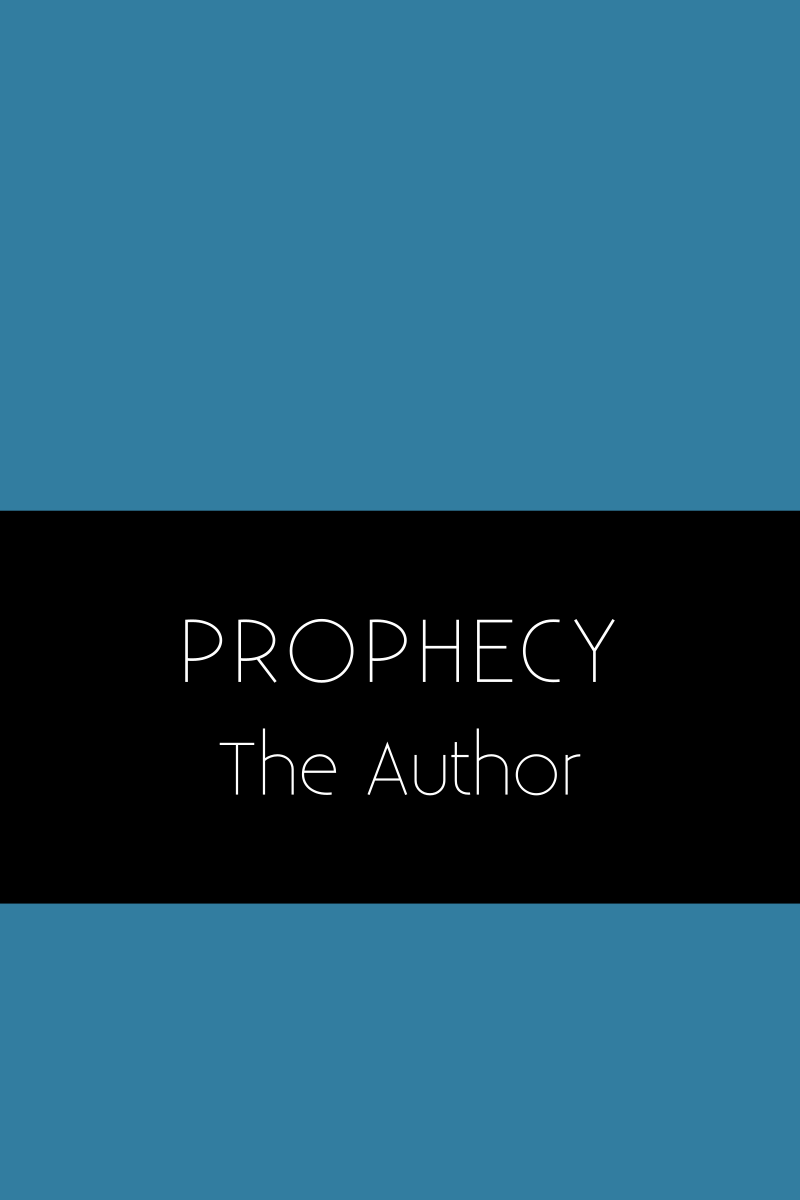
\includegraphics[height=\paperheight]{./desktop-cover.png}}
\fi

\cleartorecto
\thispagestyle{empty}

{\centering

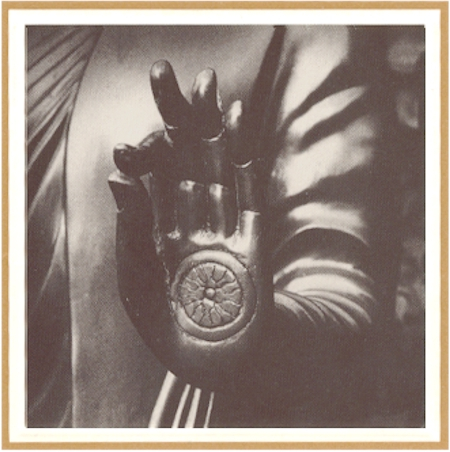
\includegraphics[width=0.7\linewidth]{image-000-mudra.jpg}

\bigskip

\settowidth{\titleLength}{%
  {\Large\chapterTitleFont\scshape\MakeLowercase{\thetitle}}%
}

{\Large\chapterTitleFont\scshape\MakeLowercase{\thetitle}}\\[0.3\baselineskip]
\setlength{\xheight}{\heightof{X}}
\raisebox{0.5\xheight}{\color[gray]{0.4}\rule{\titleLength}{0.25pt}}\\[0.3\baselineskip]
{\itshape
\thesubtitle}

\vfill

\theauthor

\vspace*{5em}

}



\cleartoverso
\thispagestyle{empty}

{\copyrightsize
\centering
\setlength{\parindent}{0pt}%
\setlength{\parskip}{0.8\baselineskip}%

\thetitle\\
por \theauthor

\emph{Perguntas e respostas baseadas nos\\
Ensinamentos do Budismo Theravāda}

Publicações Sumedhārāma\\
\href{https://sumedharama.pt}{www.sumedharama.pt}

As publicações de Sumedhārāma são para distribuição gratuita.\\
Na maioria dos casos, isto é possível graças a doações, de indivíduos ou grupos,
feitas especificamente para que as publicações dos ensinamentos do Buddha possam
estar disponíveis gratuitamente.

\textit{Sabbadānaṁ dhammadānaṁ jinati}\\
‘A oferta de Dhamma é superior a qualquer outra oferta.’

Este livro encontra-se disponível para distribuição gratuita em:\\
\href{https://sumedharama.pt}{www.sumedharama.pt}

ISBN \theISBN

Copyright \copyright\ Publicações Sumedhārāma 2024

Tradução: Dhammiko Bhikkhu\\
Formatação: Gambhīro Bhikkhu

Tradução autorizada da edição inglesa:\\
\emph{The Way It Is}\\
Amaravati Publications, 1991\\
ISBN 1-870205-11-1

\vfill

{\footnotesize

Este trabalho está licenciado com uma Licença Creative Commons\\
Atribuição-NãoComercial-SemDerivações 4.0 Internacional.

Veja página \pageref{copyright-details} para mais detalhes sobre direitos e restrições desta licença.\\
Produzido com o sistema tipográfico \LaTeX. Fonte utilizada:\\
Gentium, Crimson Roman e Cormorant.

\theEditionInfo

}}


\cleartorecto
\tableofcontents*

\chapter{Sobre o Autor}

O Venerável Ajahn Sumedho é um bhikkhu da escola Theravada de Budismo, uma
tradição que prevalece no Sri Lanka e no Sudeste da Ásia. Neste último século,
os seus ensinamentos claros e práticos foram bem recebidos no Ocidente como uma
fonte de compreensão e paz que resiste ao teste rigoroso da nossa era actual.

Ajahn Sumedho é ele próprio ocidental, tendo nascido em Seattle, Washington, EUA
em 1934. Deixou os Estados Unidos em 1964 e recebeu a ordenação de bhikkhu em
Nong Khai, no Nordeste da Tailândia em 1967. Logo a seguir, foi para o mosteiro
do Venerável Ajahn Chah, um mestre de meditação tailandês que vivia num mosteiro
na floresta conhecido como Wat Nong Pah Pong, na província de Ubon. Os mosteiros
de Ajahn Chah eram famosos pela sua austeridade e ênfase numa abordagem simples
e directa para a prática do Dhamma e Ajahn Sumedho acabou permanecendo por dez
anos neste ambiente, antes de ser convidado pelo English Sangha Trust a fixar
residência em Londres, com três outros discípulos ocidentais de Ajahn Chah.

O objectivo do English Sangha Trust era estabelecer as condições adequadas para
o treino de bhikkhus no Ocidente. A sua base em Londres, a Hampstead Buddhist
Vihara, forneceu um ponto de partida razoável, mas as vantagens de um ambiente
rural mais suave motivaram o Sangha a estabelecer um mosteiro da floresta na
Grã-Bretanha. Este objectivo foi alcançado em 1979, com a aquisição de uma casa
em ruínas, em West Sussex, que vem posteriormente a ser conhecida como Mosteiro
Budista de Chithurst ou Cittaviveka.

Com a fundação de um mosteiro adequado, o Sangha começou a aumentar de forma
constante e também assumiu o treino para mulheres como monjas budistas
(\emph{sīladhara}). O aumento do número de pessoas desejando viver a vida
monástica, ou a ajudar a sustentá-la, tornou possível o estabelecimento de
mosteiros da mesma linha na Grã-Bretanha e também no estrangeiro; igualmente
ajudou a estabelecer um centro de ensino em grande escala, o Mosteiro Budista
Amaravati, em 1984. É aqui que Ajahn Sumedho normalmente reside e onde foram
dadas muitas das palestras incluídas neste livro.

O Mosteiro Budista Amaravati fica próximo do vilarejo de Great Gaddesden, perto
de Hemel Hempstead, em Hertfordshire. É um mosteiro e centro de retiro,
acolhendo aqueles que estão interessados nos ensinamentos do Buddha. Os
visitantes podem ficar como convidados do mosteiro se estiverem interessados em
viver em comunidade e treinar em termos de moralidade, consciência e serviço.
Esta publicação faz parte do serviço que Amaravati realiza e foi disponibilizada
por meio de esforços voluntários e doações.

Amaravati produziu vários outros livros de ensinamentos de Ajahn Sumedho e
também distribuiu livros de Ajahn Chah e outros mestres budistas. Para consultar
a lista atualizada, por favor visite:

\href{https://media.amaravati.org/en/teachers/ajahn-sumedho}{https://media.amaravati.org/en/teachers/ajahn-sumedho}

\href{https://www.forestsangha.org/}{https://www.forestsangha.org/}

\clearpage

{\centering

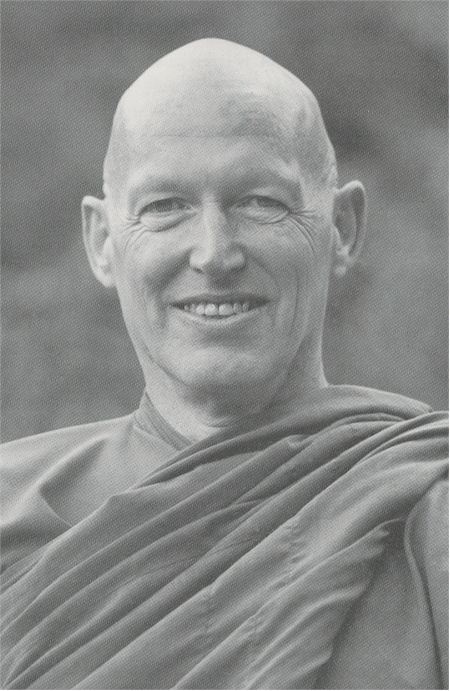
\includegraphics[width=0.8\linewidth]{image-001-aj-sumedho.jpg}

Ajahn Sumedho

\par}

\chapter{Introdução}

Este livro contém uma colecção de ensinamentos de Ajahn Sumedho dados a pessoas
que estão familiarizadas com as convenções do Budismo Theravāda e que têm alguma
experiência em meditação. A maioria dos capítulos são editados de palestras
proferidas durante retiros para leigos ou para os discípulos monásticos
(ordenados) de Ajahn Sumedho, portanto, requerem alguma atenção cuidadosa e são
melhor lidos em sequência.

Nos retiros monásticos de dois meses, Ajahn Sumedho desenvolve um tema a partir
dos ensinamentos do Buddha, ligando-o a outros aspectos do Dhamma, embelezando-o
com relatos das suas experiências pessoais, demonstrando a sua relevância para a
sociedade em geral, ou usando-o como uma exortação ao Sangha para viver de
acordo com a sua aspiração à iluminação. Embora não seja possível traduzir a
profundidade do tom e a variedade dessas palestras numa obra impressa,
acrescentada de breves exortações, directrizes e reflexões contemplativas mais
longas envolvidas com os cânticos que os monges e monjas recitam diariamente há
anos, pode sugerir a atmosfera e a perspectiva em que os ensinamentos são
oferecidos.

% REVISÃO: "Geração Dependente" — os capítulos dedicados ao tema (19–23) usam "Génese Dependente". Uniformizar o termo (recomenda-se "Génese Dependente") em todo o livro.
Em muitas dessas palestras, Ajahn Sumedho expõe a expressão singular budista de
``não-eu'' (\emph{anatta}). Ele afirma que esta é a forma do Buddha apontar para
a experiência da Realidade Última, que é o objectivo de muitas religiões.
Durante os retiros monásticos, Ajahn Sumedho frequentemente ensina a Geração
Dependente (\emph{paṭiccasamuppāda}) com base na abordagem de \emph{anatta}. A
Geração Dependente traça o processo pelo qual o sofrimento (\emph{dukkha}) é
composto pela ignorância (\emph{avijjā}) e é, inversamente, eliminado (ou
melhor, não gerado) pela cessação da ignorância. Assim como \emph{anatta},
não-eu, é a expressão da Verdade Suprema, Ajahn Sumedho sugere que a raiz da
ignorância é a ilusão de ``Eu''. É a sua tentativa de não aniquilar ou rejeitar
qualidades pessoais, mas sim indicar como o sofrimento (\emph{dukkha}) surge ao
tentar sustentar uma identidade denotada por corpo e mente.

% REVISÃO: aspas inconsistentes — usar ``Génese Dependente'' (aspas duplas, como no resto do texto) em vez de `Geração Dependente'.
% REVISÃO: vírgula a separar o sujeito do verbo ("A profundidade da ... Dependente, descreve-nos") — remover a vírgula após "Dependente"; frase de difícil leitura.
Esta identidade equivocada é o que a pessoa comum chama de ``mim''. Pode ser
detectada num estado latente como auto-consciência, como humor habitual da
mente, como vaidade, auto-criticismo, ou pode manifestar-se como actividade
egoísta corporal ou verbal. A profundidade da `Geração Dependente',
descreve-nos, como mesmo na sua forma mais passiva, essa visão errada cria
impulsos habituais (kamma) e atitudes, através das quais até mesmo um meditador
silencioso e bem-intencionado experimenta sofrimento. O Kamma vai do plano
psicológico ``interno'' até à realidade ``externa'' da acção. Este processo
habitual manifesta-se então em termos de corpo, fala ou mente; sendo todas essas
manifestações denominadas \emph{saṅkhāra}. Mesmo a acção moral baseada na
``visão egotista'', pode conduzir à ansiedade, dúvida, ``tristeza, lamento, dor,
angústia e desespero''. Esse é o significado do primeiro ``elo'' da Geração
Dependente ``\emph{avijjā paccayā saṅkhārā}'' ou ``as formações kammicas
dependem da ignorância''.

Na sua formulação mais completa, a Geração Dependente é expressa como:

\begin{quote}
  \raggedright
  Avijjā-paccayā saṅkhārā,
  saṅkhāra-paccayā viññāṇaṁ,
  viññāṇa-paccayā nāma-rūpaṁ,
  nāma-rūpa-paccayā saḷ-āyatanaṁ,
  saḷ-āyatana-paccayā phasso,
  phassa-paccayā vedanā,
  vedanā-paccayā taṇhā,
  taṇhā-paccayā upādānaṁ,
  upādāna-paccayā bhavo,
  bhava-paccayā jāti,
  jāti-paccayā jarā-maraṇaṁ soka-parideva-dukkha-domanass'upāyāsā sambhavanti.
  Evam-etassa kevalassa dukkhakkhandhassa samudayo hoti.
\end{quote}

% REVISÃO: "Isto trata-se de" é incorrecto (o sujeito de "tratar-se" é indeterminado). Corrigir para "Trata-se do surgimento de \emph{dukkha}." ou "Isto é o surgimento de \emph{dukkha}."
Isto trata-se do surgimento de \emph{dukkha}.

A cessação de \emph{dukkha} é então mapeada:

\begin{quote}
  \raggedright
  Avijjāya tveva asesa-virāga-nirodhā saṅkhāra-nirodho,
  saṅkhāra-nirodhā viññāṇa-nirodho,
  viññāṇa-nirodhā nāma-rūpa-nirodho,
  nāma-rūpa-nirodhā saḷ-āyatana-nirodho,
  saḷ-āyatana-nirodhā phassa-nirodho,
  phassa-nirodhā vedanā-nirodho,
  vedanā-nirodhā taṇhā-nirodho,
  taṇhā-nirodhā upādāna-nirodho,
  upādāna-nirodhā bhava-nirodho,
  bhava-nirodhā jāti-nirodho,
  jāti-nirodhā jarā-maraṇaṁ soka-parideva-dukkha-domanass'upāyāsā nirujjhanti.
  Evam-etassa kevalassa dukkhakkhandhassa nirodho hoti.

  \quoteRef{\href{https://suttacentral.net/sn12.35/en/bodhi}{SN 12.35, Avijjāpaccaya Sutta}}
\end{quote}

% REVISÃO: "o desejo depende da sensação; o desejo depende da sensação, a posse depende do desejo," — a vírgula após "depende do desejo" deveria ser ponto e vírgula, para manter a pontuação uniforme da enumeração.
% REVISÃO: incoerência entre os dois parágrafos — "parideva" é traduzido por "lamento" no primeiro e por "lamentação" no segundo (e "doença/morte" vs. lista distinta). Uniformizar a tradução dos termos da fórmula.
Em inglês, isto pode ser traduzido como:

\begin{quote}
  As formações habituais (kamma) dependem da ignorância; a consciência depende
  das formações habituais (kamma); o nome-forma (mentalidade-corporalidade)
  depende da consciência; as seis bases dos sentidos dependem do nome-forma; o
  contacto depende das seis bases dos sentidos; a sensação depende do contacto;
  o desejo depende da sensação; a posse depende do desejo, o devir depende da
  posse; o nascimento depende do devir; do nascimento dependem: a velhice, a
  doença e a morte, a tristeza, lamento, dor, angústia e desespero.

  Através de toda a cessação desta ignorância, cessam as formações habituais;
  através da cessação das formações habituais, cessa a consciência; através da
  cessação da consciência, cessa o nome-forma; através da cessação do
  nome-forma, cessam as seis bases dos sentidos; através da cessação das seis
  bases dos sentidos, cessa o contacto; através da cessação do contacto, cessa a
  sensação; através da cessação da sensação, cessa o desejo; através da cessação
  do desejo, cessa o apego; através da cessação do apego, cessa o devir; através
  da cessação do devir, cessa o nascimento; através da cessação do nascimento,
  cessam a velhice, a doença e a morte, a tristeza, a lamentação, a dor, a
  angústia e o desespero. Assim é a cessação de toda esta massa de sofrimento.
\end{quote}

Existem muitas formas de dependência em questão nesta análise. É útil lembrar
que \emph{paccayā} ``dependente de'' ou ``condições'' não significa
necessariamente ``gerar''. Por exemplo, poderia dizer-se ``andar depende das
pernas'', ou ``o gelo depende da água'', ou ``apanhar o comboio depende de
chegar à estação à hora certa'', ou mesmo ``a vista depende do não aparecimento
de objectos intervenientes''. Compreendendo isto, o contemplativo começa a
perceber que, assim como ``dependência emergente'' não significa necessariamente
``geração'', a ``cessação'' tão valorizada pelo Buddha não significa
necessariamente ``aniquilação''. Nesta vida, onde o Nibbāna deve ser
% REVISÃO: "formações-karmicas" — usar "kámmicas"/"kammicas" (de "kamma"), como em "formações kammicas" mais acima; evitar o hífen e a grafia "karmicas".
% REVISÃO: vírgula a separar o sujeito do verbo ("a identificação ... mentais, pode cessar") — remover a vírgula antes de "pode".
realizado, a mentalidade-corporalidade pode ``cessar'' -- ou seja, a
identificação com as formações-karmicas físicas e mentais, pode cessar de
modo a que a vida não seja mais vivida a partir do princípio do prazer/dor
ditado pelos sentidos. (\emph{nāma-rūpa-saḷāyatana-phassa-vedanā-taṇhā}). Com
este espírito, pode-se interpretar a sequência de uma forma mais fluida, por
exemplo:

% REVISÃO: "objeto" deveria ser "objecto" (grafia pré-Acordo, como no resto do livro).
Na medida em que (\emph{paccayā}) a mente não compreendeu (\emph{avijjā}) a
Verdade, impulsos habituais (\emph{saṅkhārā}) manifestam e condicionam
(\emph{paccayā}) a consciência para um modo discriminativo (\emph{viññāṇa}) que
opera em termos de (\emph{paccayā}) sujeito e objeto (\emph{nāma-rūpa}) mantidos
(\emph{paccayā}) para existir num lado ou outro das seis portas dos sentidos
(\emph{saḷāyatana}).

% FIXME: domanassa missing

Estas portas dos sentidos abrem-se dependendo (\emph{paccayā}) do contacto
(\emph{passā}) que pode suscitar (\emph{paccayā}) vários graus de sensação
(\emph{vedanā}). A sensação estimula (\emph{paccayā}) o desejo (\emph{taṇhā}) e,
de acordo com (\emph{paccayā}) o poder do desejo, a atenção mantém-se
(\emph{upādāna}) e assim se desenvolvem objectivos e obsessões pessoais
(\emph{bhava}) que dão (\emph{paccayā}) o ciclo de amadurecimento e
desaparecimento (\emph{jarā-maraṇa}) com o resultante sentimento de tristeza
(\emph{soka}) variando entre angústia (\emph{parideva}), depressão
(\emph{dukkha}) e esgotamento nervoso (\emph{upāyāsa}).

Quando a mente olha para o sentimento de perda e compreende a Verdade
\emph{(avijjā-nirodha)}, os impulsos habituais cessam \emph{(saṅkhāra-nirodha)}
e a consciência não mais é limitada pela discriminação dos mesmos
\emph{(viññāṇa-nirodha)}, de modo que a separação entre sujeito e objecto não
mais é sustentada \emph{(nāma-rūpa nirodha)} e não nos sentimos encurralados
dentro ou puxados para fora das seis portas dos sentidos
\emph{(saḷāyatana-nirodha)}. As portas dos sentidos abrem-se à reflexão, ao
invés de ficarem dependentes do contacto \emph{(phassa-nirodha)} e o impacto não
se imprime adentro na mente (\emph{vedanā-nirodha}). Portanto, existe liberdade
em relação ao desejo \emph{(taṇhā-nirodha)} e a atenção não fica presa
\emph{(upādāna-nirodha)} nem cresce para motivações egoístas
\emph{(bhava-nirodha)} que reforçam e se centram no ego. Quando nenhuma imagem
pessoal é criada, jamais poderá inflar nem ser destruída
\emph{(jarā-maraṇa-nirodha)}. Assim, nada há a perder, permanecendo uma sensação
de felicidade, elevação, alegria e serenidade
\emph{(soka-parideva-dukkha-domanassa-upāyāsā-nirodha)}.

Com a cessação de tal ponto de referência limitado à morte, passa-se a viver a
Verdadeira vida, a vida Santa, da qual Ajahn Sumedho tão evocativamente fala.

Embora muitas destas palestras tenham sido dadas para monásticos, a beleza do
Dhamma é estar disponível para aqueles que desejam ouvir. É com isto em mente
que este livro é oferecido gratuitamente.

\bigskip

{\raggedright
  Que todos os seres realizem a Verdade,\\
  Ven. Sucitto Bhikkhu\\
  Amaravati
\par}


% Page 1 is the first page of the first chapter.
\mainmatter

\chapter{``\ldots{} Felicidade para sempre''}

\ldots{} Temos meditado, observando a nossa respiração, contemplando a inalação
e a exalação. Estamos a usar a atenção pura, consciência do corpo enquanto
caminhamos, de pé, sentados e deitados. Em vez de nos fascinarmos, estamos a
abrir a mente às condições tal como estão no presente momento.

Reparai como até num lugar bonito como este, podemos mesmo tornar a nossa vida
miserável. Quando estamos aqui, talvez queiramos estar num outro lugar qualquer;
quando estamos a andar, podemos querer estar sentados; quando estamos sentados,
talvez queiramos andar. Quando estamos a meditar, estamos a pensar no que vamos
fazer depois do retiro. E então, depois do retiro, gostaríamos de voltar\ldots{}
incorrigível, não é?

Quem sabe antes de virem para este retiro, estavam a ter problemas em casa e
pensavam: ``Mal posso esperar para ir para o retiro''. E depois aqui desejam:
``Mal posso esperar que o retiro acabe.'' Ou talvez se tranquilizem imenso aí
sentados a pensar: ``Quero estar sempre assim'', ou tentam obter aquele estado
arrebatador que obtiveram ontem, mas em vez disso irritam-se cada vez mais.

Quando obtemos estes estados agradáveis de arrebatamento, agarramo-nos a eles;
mas depois temos que arranjar algo para comer, ou fazer algo. Sentimo-nos então
mal ao perdermos o estado arrebatador. Ou talvez não tenhamos tido quaisquer
estados arrebatadores: surgem apenas muitas memórias miseráveis, raiva e
frustrações. Todas as outras pessoas estão felicíssimas; então sentimo-nos
chateados porque toda a gente parece estar a receber alguma coisa deste retiro,
excepto nós\ldots{}

É assim que começamos a observar que tudo muda. Depois temos a possibilidade de
observar como criamos problemas ou nos apegamos ao bem ou criamos todo o tipo de
complexidades em torno das condições do momento; querendo algo que não temos,
querendo manter algo que temos, querendo nos livrar de algo que temos. Este é o
problema humano do desejo, não é? Estamos sempre à procura de outra coisa.

Lembro-me de quando era criança querer um certo brinquedo. Disse à minha mãe que
se tivesse aquele brinquedo, nunca mais quereria nada. Satisfar-me-ia
completamente. E eu acreditava naquilo -- não lhe estava a dizer mentira
nenhuma; a única coisa que me impedia de realmente ser feliz naquele momento era
eu não ter o brinquedo que queria. Então a minha mãe comprou o brinquedo e
deu-mo. Consegui retirar alguma felicidade do brinquedo durante uns 5 minutos
talvez\ldots{} e então tive que começar a querer outra coisa. Portanto, ao
obter o que eu queria, senti alguma gratificação e felicidade e então o desejo
por algo mais surgia. Lembro-me disto tão vividamente porque naquela idade tão
jovem, eu realmente acreditava que se tivesse aquele brinquedo que eu queria,
seria feliz para sempre\ldots{} simplesmente para depois compreender que
``felicidade para sempre'' era uma impossibilidade\ldots{}

\photoPage{image-002-bhikkhu-meditating.jpg}{Um Bhikkhu a meditar no exterior do seu kuti}{Foto por John Johns}

\chapter{Investigando a Mente}

\lettrine{A}{raiz do sofrimento} é o que chamamos \emph{avijjā} -- o não saber, ou a ignorância de
como realmente as coisas são. Esta ignorância básica é aquela de não compreender
a nossa verdadeira natureza. Sofremos por causa de maneiras de ver e opiniões, e
por causa de hábitos e condições que não compreendemos. Vivemos as nossas vidas
num estado de ignorância, não compreendendo a forma como as coisas são.

Se nos ouvirmos muito, por vezes podemos ouvir declarações tais como: ``Eu devia
fazer isto, eu não devia fazer isto, eu devia ser assim, eu não devia ser
assim'', ou que o mundo seria diferente do que é; os nossos pais deveriam ser
desta ou daquela maneira e não deviam ser como são. Então, temos este tempo
verbal em particular a ressoar na nossa cabeça porque temos uma ideia do que
deveria ou não deveria ser. Na meditação, escutem aquela opinião dentro de vós
do que deveria e não deveria ser -- simplesmente escutem-na.

A nossa tendência é tentar tornarmo-nos algo; então estabelecemos um objectivo,
criamos um ideal do que gostaríamos de nos tornar. Talvez pensemos que a
sociedade deve ser diferente do que é. As pessoas deviam ser amáveis, generosas,
altruístas, compreensivas e amorosas; devia haver fraternidade e as pessoas não
deviam ser egoístas. O governo devia ter líderes sábios, o mundo devia estar em
paz e assim por diante. Mas o mundo está como está neste momento e as coisas são
como são. Quando não compreendemos isto, então debatemo-nos. Assim, ouçam
interiormente o choro constante. ``Eu sou assim, eu não sou assim'', e penetrem
neste ``eu sou, eu não sou'' com consciência.

Temos tendência para reagir e assumir por garantido que todo o ``eu sou'' e
``não sou'' é a verdade. Criamo-nos como uma personalidade e apegamo-nos às
nossas memórias. Lembramo-nos das coisas que aprendemos e do que fizemos --
geralmente as coisas mais extremas; temos tendência para esquecer as coisas mais
comuns. % REVISÃO: "Pessoas que viveram vidas muito egoístas, têm de beber" — a vírgula separa indevidamente o sujeito do verbo; deve ser removida.
Portanto, se fizermos coisas indelicadas, cruéis e tolas, então temos
memórias desagradáveis nas nossas vidas; sentimo-nos envergonhados ou culpados.
Se fizermos coisas boas ou caridosas, então temos boas memórias nas nossas
vidas. Quando começarmos a reflectir sobre esta questão, então teremos mais
cuidado com o que fazemos e dizemos; se tivermos vivido a vida
inconscientemente, agindo impulsivamente por desejo de gratificação imediata ou
por uma intenção de magoar, causar desarmonia ou explorar os outros, as nossas
mentes estarão cheias de memórias muito desagradáveis. Pessoas que viveram vidas
muito egoístas, têm de beber muito ou tomar drogas para se manterem
constantemente ocupadas, de forma a não terem que olhar para as memórias que
surgem na mente.

No processo de despertar na meditação, estamos a trazer consciência para as
condições da mente aqui e agora só por estarmos conscientes desta noção de ``eu
sou, não sou''. Contemplemos os sentimentos de dor ou prazer -- e quaisquer
memórias, pensamentos e opiniões -- como impermanentes, \emph{anicca}. A
característica do transitório é comum a todas as condições. Quantos de vós
passaram o dia a investigar isto de todas as formas possíveis enquanto sentados,
de pé ou deitados? Investiguem o que vêem através dos olhos, o que ouvem através
dos ouvidos, o que saboreiam com a língua, cheiram com o nariz, sentem e
experimentam com o corpo e pensam com a mente.

O pensamento ``eu sou'' é uma condição impermanente. O pensamento ``não sou'' é
uma condição impermanente. Pensamentos, memórias, consciência do pensamento, o
próprio corpo, as nossas emoções -- todas as condições mudam. Na prática da
meditação, temos de assumir bastante seriedade, bravura e coragem para realmente
investigarmos, ousar olharmos até para as condições mais desagradáveis da vida,
em vez de procurarmos uma fuga na tranquilidade ou de esquecermos tudo. Em
\emph{Vipassana}, a prática é a de olhar para dentro do sofrimento; é um
confronto connosco mesmos, com o que pensamos de nós mesmos, com as nossas
memórias e emoções, agradáveis, desagradáveis ou indiferentes. Por outras
palavras, quando estas coisas surgem e estamos conscientes do sofrimento, em vez
de o rejeitarmos, reprimirmos ou ignorá-lo, aproveitamos a oportunidade para o
examinar.

Então o sofrimento é o nosso professor. Ensina-nos e por isso temos de aprender
a lição através do estudo do próprio sofrimento. Surpreende-me sempre como
algumas pessoas pensam que nunca sofrem. Pensam: ``Não sofro. Não sei porque é
que os budistas estão sempre a falar de sofrimento. Sinto-me maravilhoso, cheio
de beleza e alegria. Estou sempre tão feliz. Acho a vida uma experiência
fantástica, interessante, fascinante e um prazer interminável''. Estas pessoas
têm tendência para aceitar esse lado da vida e rejeitar o outro, porque
inevitavelmente o que nos encanta desaparece e depois lamentamos.

% REVISÃO: "O nosso desejo ... de deleite, leva-nos" — a vírgula separa o sujeito do verbo; deve ser removida.
O nosso desejo de estar num constante estado de deleite, leva-nos a todo o tipo
de problemas, dificuldades e situações. O sofrimento não existe só por causa de
coisas gravíssimas como ter cancro terminal, ou perder alguém que se ama; o
sofrimento pode ocorrer em torno do que é muito comum, como as quatro posturas,
sentar, ficar de pé, andar, deitar-se. Não há nada de extremo nisso.

Contemplamos a respiração normal e a consciência corrente. De forma a
compreender a existência, contemplamos sentimentos, memórias e pensamentos
comuns em vez de procurarmos agarrar ideias e pensamentos fantásticos para
compreendermos os extremos da existência. Assim não nos estamos a envolver com
especulações sobre o propósito final da vida, Deus, o diabo, o céu, o inferno e
o que acontece quando morremos ou reencarnamos. Na meditação budista, só
observamos o aqui e agora. O nascimento e morte que está a acontecer aqui e
agora é o começo e o fim das coisas mais comuns.

Contemple-se o início. Quando se pensa em nascimento, pensa-se em ``Eu nasci'',
mas esse é o grande nascimento do corpo, que não nos conseguimos lembrar. O
nascimento comum de ``eu'' que vivenciamos na vida diária é ``eu quero, eu não
quero, eu gosto, eu não gosto''. Isto é um nascimento, ou busca de ser feliz.
Contemplamos o comum inferno da nossa própria raiva, a raiva que surge, o calor
do corpo, a aversão, o ódio que sentimos na mente. Contemplamos o paraíso comum
que experimentamos, os estados felizes, a bem-aventurança, a leveza, a beleza no
aqui e agora. Ou apenas o estado mental embotado, o tipo de limbo, nem feliz nem
infeliz, mas embotado, entediado e indiferente. Na meditação budista, observamos
isto dentro de nós mesmos.

Contemplamos o nosso próprio desejo de poder e controlo, de controlar outro
alguém, de nos tornarmos famosos ou de nos tornarmos alguém que está no topo.
Quantos de vós, quando descobrem que alguém é mais talentoso do que vocês,
querem colocá-lo para baixo? Isso é ciúme. O que temos que fazer na nossa
prática de meditação é ver os ciúmes típicos, ou o ódio que podemos sentir por
alguém que pode aproveitar-se de nós ou incomodar-nos; a ganância ou luxúria que
podemos sentir por alguém que nos atrai. A nossa própria mente é como um espelho
que reflecte o universo e nós observamos o reflexo. Antes, assumiríamos esses
reflexos como realidade de modo a ficarmos fascinados, enojados ou indiferentes
a eles. Mas em \emph{Vipassana}, apenas observamos que todas essas reflexões são
condições mutáveis. % REVISÃO: "onde quando como ignorantes" está truncado/agramatical. Reformular, p. ex.: "ao passo que, como ignorantes, temos a tendência para procurar identidade nelas."
Começamos a vê-las como objectos em vez de um eu, onde
quando como ignorantes, temos a tendência para procurar identidade nelas.

% REVISÃO: concordância de tempos verbais — "sentar-se-á ... e experimentará ... até mesmo cheirar odores ... e ouvir sons divinos e pense:" mistura futuro e infinitivo. Uniformizar no futuro: "cheirará ... ouvirá ... e pensará:".
% REVISÃO: "Por que algo assim nunca acontece comigo?" — construção do português do Brasil; em PT-PT preferir "Porque é que algo assim nunca me acontece?".
Portanto, na prática, estamos a olhar para o universo conforme ele está a ser
reflectido nas nossas mentes. Não importa o que os outros experimentem; um
meditador sentar-se-á aqui e experimentará todos os tipos de luzes brilhantes,
cores, imagens fascinantes, Buddhas, seres celestiais, até mesmo cheirar odores
maravilhosos e ouvir sons divinos e pense: ``Que meditação maravilhosa, veio
tanto brilho, `o esplendor' -- um ser divino veio como um anjo esplendoroso,
tocou-me e senti este êxtase. A experiência de êxtase mais maravilhosa de toda a
minha vida\ldots{} Esperei toda a minha vida por esta experiência.'' Enquanto
isso, o próximo está a pensar: ``Por que algo assim nunca acontece comigo?
Sentei-me durante uma hora inteira com dores nas costas, deprimido, com vontade
de fugir, perguntando-me por que raio vim eu a este retiro''. Outra pessoa
poderá dizer: ``Eu não aguento todas aquelas pessoas que têm aquelas ideias
parvas e fantasias. Elas metem-me nojo; provocam-me este terrível ódio e aversão
em mim. Eu odeio a imagem do Buddha sentado na janela. Quero esmagá-la. Eu odeio
o Budismo e a meditação!''

% REVISÃO: "alguém que vê \emph{devas} e experiência luzes brilhantes" e "do êxtase ou experiência entorpecimento" — aqui "experiência" é forma verbal e deve escrever-se "experiencia" (sem acento, do verbo experienciar).
Agora, qual dessas três pessoas é o bom meditador? Compare-se com aquele que vê
\emph{devas} a dançar no céu, aquele que está aborrecido, indiferente e
embotado, ou aquele cheio de ódio e aversão? \emph{Devas} e anjos a dançar nos
reinos celestiais são \emph{anicca}, são impermanentes. O aborrecimento é
\emph{anicca}, impermanente. O ódio e a aversão são \emph{anicca},
impermanentes. Portanto, o bom meditador, aquele que pratica da maneira certa vê
a natureza impermanente destas condições. Quando fala com alguém que vê
\emph{devas} e experiência luzes brilhantes, começa a duvidar da sua própria
prática e pensa: ``Talvez eu não seja capaz de iluminação. Talvez eu não esteja
a meditar como deve ser''. A dúvida é em si impermanente. Tudo o que surge
passa. Portanto, o bom meditador é aquele que vê a natureza impermanente da
bem-aventurança e do êxtase ou experiência entorpecimento, raiva, ódio e aversão
e reflecte sobre a natureza impermanente dessas qualidades quando medita
sentado, a caminhar ou deitado.

Qual é a sua tendência? É muito optimista sobre tudo? ``Eu gosto de todos aqui.
Eu acredito nos ensinamentos do Buddha, eu acredito no Dhamma'' -- esse tipo de
mente é de fé, acredita. E este tipo de mente pode criar e experienciar muito
rapidamente coisas arrebatadoras. Alguns dos agricultores na Tailândia, pessoas
quase sem conhecimento algum sobre as coisas do mundo, que mal sabem ler e
escrever, às vezes podem experienciar estados de felicidade, luzes, \emph{devas}
e tudo mais, e acreditar neles. Quando acreditamos em \emph{devas}, vemo-los.
Quando acreditamos em luzes e reinos celestiais, iremos vê-los. Acreditamos que
Buddha virá salvar-nos, Buddha virá e salvar-nos-á. Aquilo em que acreditamos,
acontece connosco. Se acreditamos em fantasmas, fadas e elfos, veremos que estas
coisas se manifestam para nós. Mas ainda são \emph{anicca}, impermanentes,
transitórios e não-eu.

A maioria das pessoas não acredita em fadas e \emph{devas} e pensam que tais
coisas são uma idiotice. Esse é o tipo de mente negativa, que é desconfiada e
duvidosa e que não acredita em nada. ``Eu não acredito em fadas e \emph{devas}.
Eu não acredito em nada desse género de coisas. Ridículo? Mostre-me uma fada.''
Portanto, a mente muito desconfiada e céptica nunca vê tais coisas.

A fé existe; a dúvida existe. Na prática budista, examinamos a crença e a dúvida
que experienciamos na nossa mente e vemos que estas duas condições estão a
mudar.

Já contemplei a própria dúvida como um sinal. Eu fazia a mim próprio uma
pergunta como, ``Quem sou eu?'' E então ouvia a resposta -- algo como, ``Sumedho
Bhikkhu''. Então pensava: ``Esta não é a resposta; quem és tu realmente?'' Eu
veria o conflito, a habitual reacção para encontrar uma resposta para a
pergunta. Mas eu não aceitaria qualquer resposta conceitual. ``Quem está aqui
sentado? O que é isto? O que é isto aqui? Quem está pensando, afinal? O que é
que pensa?'' Quando um estado de incerteza ou dúvida surgisse, eu apenas olharia
para essa incerteza ou dúvida como um sinal, porque a mente pára aí e fica em
branco, e então surge o vazio.

Achei útil esvaziar a mente perguntando a mim mesmo perguntas irrespondíveis que
fariam com que surgissem dúvidas. A dúvida é uma condição impermanente. A forma,
o conhecido, é impermanente; não saber é impermanente. Alguns dias eu saía e
olhava a natureza e observava-me apenas parado aqui, olhando para o chão. Eu
perguntar-me-ia: ``O solo está separado de mim? Quem é este que vê o chão? \ldots{}
Estas folhas e o solo estão na minha mente ou fora da minha mente? \ldots{} O que é
isso que vê? É o globo ocular? \ldots{} Se eu arrancasse o meu globo ocular, ele
seria separado de mim? \ldots{} Eu ainda veria essas folhas? \ldots{} Eles ainda ali estão
quando não estou a olhar para eles? \ldots{} Quem é que está ciente disso, afinal?''

E o som. Também fiz algumas experiências com som porque os objectos da visão têm
uma certa solidez como esta sala -- parece bastante permanente, sabe, pelo menos
por hoje. Mas o som é verdadeiramente \emph{anicca} -- tente controlar o som.

Investiguei o som perguntando: ``Os meus olhos podem ouvi-lo? Se eu cortar os
meus ouvidos e tímpanos, haverá algum som? Posso ver e ouvir exactamente no
mesmo momento?'' Todos os órgãos dos sentidos e os seus objectos são
impermanentes, mudando as condições. Pense agora: ``Onde está a sua mãe? Onde
está a minha mãe agora?'' Se eu pensar nela no seu apartamento na Califórnia, é
um conceito na mente. Mesmo se eu pensar, ``A Califórnia é ali'', ainda é a
mente a pensar ``ali''. ``Mãe'' é um conceito, não é? Então, onde está a mãe
agora? Ela está na mente: quando a palavra ``mãe'' surge, você ouve a palavra
como um som e ela traz uma imagem mental ou uma memória ou um sentimento de
gosto, antipatia ou indiferença.

% REVISÃO: "Você tem preconceitos e preconceitos sobre raça ou nacionalidade" — palavra repetida; o original distingue dois termos (p. ex. "ideias preconcebidas e preconceitos").
% REVISÃO: "isto é só inerente nessas identidades" — regência incorrecta; "inerente" rege a preposição "a": "inerente a essas identidades".
Todos os conceitos na mente que consideramos realidade devem ser investigados:
saiba o que os conceitos fazem à mente. Observe o prazer que obtém ao pensar em
certos conceitos e o desprazer que outros trazem. Você tem preconceitos e
preconceitos sobre raça ou nacionalidade -- todos estes são conceitos ou
proliferações conceituais. Os homens têm certas atitudes e preconceitos em
relação aos homens: isto é só inerente nessas identidades.

Mas na meditação, ``feminino'' é um conceito e ``masculino'' é um conceito, um
sentimento, uma percepção na mente. Portanto, nesta prática de \emph{Vipassana},
penetramos com discernimento na natureza de todas as condições, grosseiras ou
subtis. A compreensão interior destrói as ilusões que estes conceitos nos dão,
de serem reais. Podem surgir condições; não podemos parar as coisas que nos
afectam na vida -- como o clima, a economia, problemas familiares, o nosso
passado, a nossa oportunidade ou falta de oportunidade. Mas podemos penetrar em
todas estas condições -- que são impermanentes e não-eu. Este é o caminho da
transcendência; transcendendo a condição mortal através da consciência da
condição mortal.

O Buddha é o professor, aquilo que dentro de nós nos lembra de observar a
natureza impermanente de todas as condições e a não assumir nenhuma delas como
realidade. Quando o fazemos, o que acontece? Temos guerras, greves, batalhas e
problemas sem fim que existem no mundo porque os seres ignorantes assumem essas
condições como realidade. Ligam-se ao corpo mortal como uma identidade. Somos
absorvidos nestes vários símbolos e conceitos e, nessa absorção, temos que
nascer e morrer nessas condições. É como apegarmo-nos a algo que está a
mover-se, como a ganância e ser puxado por esse movimento. Então, nascemos e
morremos nesse momento. Mas quando não nos apegamos mais, então estamos a evitar
sofrer do movimento e das limitações da mudança de condições.

Ora, falando assim, as pessoas podem questionar: ``Mas como viver então nesta
sociedade, se tudo é irreal?'' O Buddha fez uma distinção muito clara entre a
realidade convencional e a realidade última. No nível convencional de
existência, usamos convenções que trazem harmonia para nós mesmos e para a
sociedade em que vivemos. Que tipo de convenções trazem harmonia? Bem, coisas
como ser bom, estar atento, não fazer coisas que causam desarmonia, como roubar,
enganar e explorar os outros. Ter respeito e compaixão pelos outros seres, ser
observador, tentar ajudar: todas estas convenções trazem harmonia.

Portanto, no ensino Budista ao nível convencional, vivemos de uma maneira que
apoia a prática do bem e evitamos fazer o mal com o corpo e a fala. Não é como
se estivéssemos a rejeitar o mundo convencional ``Não quero ter nada a ver com
isso porque é uma ilusão'' -- isso é \emph{outra} ilusão. Pensar que o mundo
convencional é uma ilusão é só mais um pensamento.

Na nossa prática, nós vemos que pensamento é pensamento, ``o mundo é uma
ilusão'' é um pensamento. Mas aqui e agora, devemos estar cientes de que tudo o
que temos consciência está a mudar. Vivam conscientemente, ponham esforço e
concentração no que fazem, estejam sentados, a andar, deitados ou a trabalhar.
Independentemente de se ser homem ou mulher, um secretário, secretária, dona de
casa ou trabalhador, executivo, ou seja, o que for, requer esforço e
concentração. Fazer o bem e evitar fazer o mal. Isto é como um budista vive
dentro das formas convencionais da sociedade. Mas não mais iludidos pelo corpo
ou pela sociedade, ou pelas coisas que se passam na sociedade, porque uma pessoa
budista é aquela que examina e investiga o universo ao investigar o seu próprio
corpo e mente.

\chapter{Tudo o Que Surge Acaba}

\lettrine{O}{\space Buda disse que} a origem de todo sofrimento é a ignorância -- por isso é
importante considerar o que ele realmente quis dizer por ``ignorância''. Na sua
maioria, os seres humanos no mundo vivem como se realmente fossem os seus
próprios hábitos, pensamentos, sentimentos e memórias. Não usam o tempo ou não
têm a oportunidade de olhar para as suas vidas, de observarem e considerarem
como estas condições funcionam.

O que é uma condição? O corpo com o qual estamos, as emoções e sentimentos, as
percepções da mente, concepções e consciência através dos sentidos -- estas são
as condições. Uma condição é algo que é adicionado e composto; algo que surge e
acaba; não é o incriado, não nascido, a realidade última não originada.

A religião é o que os seres humanos usam para tentarem regressar à realização
última para além dos ciclos de nascimento e morte, a sabedoria supramundana ou
\emph{lokuttara paññā}; Nirvāna ou Nibbāna é a experiência dessa
realidade transcendente. Isto é quando subitamente conhecemos a verdade, não por
estudar as escrituras Pāli ou um livro Zen, mas por experiência directa.

Geralmente concebemos a verdade como sendo \emph{algo} e Nibbāna como
sendo um estado mental pacífico ou experiência extática. Todos nós já
experimentámos algum tipo de felicidade, então gostamos de conceber o Não
Nascido, Incriado, Não Originado como uma experiência feliz. Mas o Buddha foi
muito cuidadoso em nunca descrever a Realidade Suprema ou Nibbāna -- ele
nunca falou muito sobre isso. As pessoas querem saber o que é, escrever livros
sobre isso e especular sobre a natureza do Nibbāna -- mas isso é
exactamente o que o Buddha não fez.

Em vez disso, ele apontou para o conhecimento directo das condições que mudam,
aquilo que podemos saber pela nossa própria experiência neste momento. Não se
trata de acreditar em qualquer outro alguém. É uma questão de saber, neste
momento presente, que tudo o que surge acaba.

Portanto, colocamos esse tipo de atenção nas nossas vidas -- para estarmos
atentos e percebermos que tudo o que surge acaba; que qualquer condição da nossa
mente ou corpo -- seja uma sensação de prazer ou dor, sentimento ou memória,
visão, som, cheiro, paladar ou tacto, dentro ou fora -- é apenas uma condição.

É importante reflectir sobre o significado real de ``ignorância'' no sentido em
que o Buddha disse quando lhe chamou a origem de todo sofrimento. ``Ser
ignorante'' significa que nos identificamos com essas condições, considerando-as
como ``eu'' ou ``meu'' ou como algo que não queremos ser ``eu'' ou ``meu''.
Temos a ideia de que temos que encontrar alguma condição agradável permanente,
conseguir algo, obter algo que não temos. Mas podemos perceber que o desejo na
mente é uma coisa em movimento; está à procura de algo, portanto é uma condição
em mudança que surge e acaba -- é não-eu (não é eu). A expressão ``não-eu''
(\emph{anatta}) não é um tipo qualquer de mantra\footnote{Uma palavra ou frase
  com significado espiritual. É usado como um foco de atenção e reflexão ao se
  repetir muitas vezes na meditação.} que usamos para nos livrarmos das coisas,
mas é uma penetração real compreensiva da natureza básica de todos os desejos.

Ao olhar com cuidado, com muita paciência e humildade, começamos a ver que o
criado surge do Incriado e volta ao Incriado; desaparece e nada mais resta. Se
fosse realmente eu e realmente meu, ficaria, certo? Se fosse realmente meu, para
onde iria, para algum tipo de arrecadação de personalidade? Mas esse conceito e
tudo o que se possa conceber é uma condição que surge e acaba. Sempre que nos
tentamos conceber, qualquer conceito ou memória de nós como isto ou aquilo é
apenas uma condição da nossa mente. Não é o que somos -- nós não somos uma
condição da nossa mente. Então, tristeza, desespero, amor e felicidade são todas
condições da mente e são todas não-eu.

Observemos na nossa vida quando sofremos ou sentimos descontentamento -- porquê?
É por causa de algum apego, alguma ideia de nós ou de outra pessoa. Alguém que
amamos morre e sentimos pena de nós mesmos; pensamos nos bons momentos que
tivemos e concentramo-nos nisso, criando mais condições da mente. Talvez
sintamos culpa por não termos dado ou amado o tempo inteiro -- sendo esta também
uma condição da mente. Temos uma memória; concebemo-los como estando vivos --
mas a própria ideia de uma pessoa é uma percepção da mente -- não uma pessoa, ou
é? Lembramo-nos de alguém ainda vivo, com quem gostaríamos de estar agora -- essa
é uma condição da mente; ou lembramo-nos de alguém que morreu, que jamais
veremos -- isso também é uma condição da mente.

A meditação budista é uma forma de ver as condições da mente, investigando e
vendo o que são, em vez de acreditar nelas. As pessoas querem acreditar --
quando alguém próximo de nós morre, alguém acaba por nos dizer: ``Oh, subiu ao
céu com Deus Pai'', ou ``estão agora a viver nas delícias do céu Tusita.'' Dizem
isto de forma a termos uma percepção agradável mental -- ``Bem, agora sei que a
minha avó está feliz lá em cima nos reinos celestiais, dançando com os anjos''.
Então, outro alguém diz ``Bem, sabe, ela fez algumas coisas bem más, ela
provavelmente está lá em baixo no Inferno, ardendo nos fogos eternos!'' Com
isto, logo nos começamos a preocupar que igualmente lá acabemos talvez -- mas
isso é uma percepção da mente. Céu e Inferno são fenómenos condicionados. Então
-- se reflectirmos sobre algo sucedido há dez anos\ldots{} essa é uma condição da
mente que surge e acaba, e a razão porque surge é porque eu acabei de a sugerir.
Portanto, essa condição depende de outra condição, a memória é o que
experienciámos e o futuro é o desconhecido.

Mas quem é que conhece as condições do momento? Não o consigo encontrar: só o
saber existe, e o saber pode conhecer tudo o que está presente agora --
agradável ou desagradável -- especulações sobre o futuro ou reminiscências do
passado -- criações de nós mesmos como isto ou aquilo. Criamo-nos a nós mesmos
ou ao mundo em que vivemos -- então não podemos realmente culpar mais ninguém.
Se o fazemos, é porque ainda somos ignorantes. Denominamos ``Aquele que Sabe''
de ``Buddha'' -- mas isso não significa que ``Buddha'' seja uma condição. Não é
dizer que esta Buddha-rupa (estátua de Buddha) saiba alguma coisa; mais do que
isso, significa que ``Buddha'' é o saber. Portanto, a meditação budista é
realmente estar ciente, mais do que se tornar Buddha.

A ideia de nos tornarmos Buddha é baseada em condições -- pensamos ser alguém
que agora não é Buddha, e de forma a nos tornarmos Buddha temos que ler livros
para descobrir como nos tornaremos num. Claro, isso significa que temos que
trabalhar muito para nos livrarmos das qualidades que não são características de
Buddha; estamos longe de ser perfeitos, irritamo-nos, somos gananciosos,
duvidosos e amedrontados, e claro, os Buddhas não têm isto -- porque Buddha é
aquilo que sabe, portanto eles sabem melhor. Então, para nos tornarmos Buddha,
temos que nos livrar dessas coisas que não são características de Buddha e
tentar obter qualidades características de Buddha como compaixão e todos estes
tipos de coisas. \emph{E tudo isto são criações da mente!} Portanto, criamos
``Buddhas'' porque acreditamos nas criações da mente. Mas elas não são Buddhas
reais. Elas são apenas falsos Buddhas. Eles não são Buddhas de sabedoria, são
apenas condições da nossa mente.

Enquanto nos concebermos como alguém que tem que fazer algo para se tornar outra
coisa, ainda caímos numa armadilha, uma condição da mente como sendo um eu, e
nunca entenderemos nada como deve ser. Independentemente de quantos anos
meditemos, nunca realmente entenderemos o ensinamento; simplesmente falharemos
sempre o alvo. A maneira directa de ver as coisas \emph{agora} -- de que tudo o
que surge acaba -- não significa que estamos a desprezar o que seja. Significa
que estamos a observar de uma maneira que nunca nos preocupámos em observar
antes. Estamos a observar de uma perspectiva daquilo que está aqui e agora, em
vez de procurar por algo que não está aqui. Então, se entramos na Sala de
Meditação a pensar: ``Eu tenho que passar esta hora a procurar pelo Buddha,
tentar tornar-me algo, tentar livrar-me destes pensamentos nefastos, sentar e
praticar duro, tentar tornar-me o que eu me deveria tornar -- então vou
sentar-me aqui e tentar livrar-me de coisas, tentar obter coisas, tentar segurar
as coisas'' \ldots{} com essa atitude, a meditação é um esforço realmente
extenuante e sempre um fracasso.

Mas, se em vez disso, entramos na Sala de Meditação e estamos simplesmente
cientes das condições da mente, vemos em perspectiva o desejo de se tornar, de
se livrar de, de fazer algo ou a sensação de que não o conseguimos fazer; ou que
se é um especialista, seja o que for -- começamos a ver que tudo o que estamos a
experienciar é uma condição que muda e não ``eu''. Observamos a perspectiva de
ser Buddha, em vez de fazer algo para nos tornarmos Buddha. Quando falamos sobre
\emph{sati}, consciência, é isto que queremos dizer.

Estou realmente chocado e surpreso com muitas pessoas religiosas -- cristãos ou
budistas ou o que seja -- que parecem ignorar a prática da sua religião. Poucas
pessoas parecem ter qualquer perspectiva sobre a doutrina religiosa, crença e
descrença. Não se preocupam em descobrir. Ainda estão a tentar descrever o
indescritível, limitar o ilimitado, conhecer o incognoscível\ldots{} e poucas
pessoas reparam na forma como se encontram. Acreditam naquilo que outro alguém
lhes disse.

Hoje em dia, monges Budistas Theravāda dir-vos-ão que vocês não se podem
iluminar, já nem podemos sequer alcançar a entrada-no-caminho (corrente), o
primeiro estágio da santidade, que esses tempos são passado. Eles acreditam que
a iluminação é uma possibilidade tão remota que já nem eles próprios sequer
colocam muito esforço para verem que tudo o que surge acaba. Portanto, os monges
podem passar vidas inteiras a ler livros e a traduzir Suttas, acreditando ainda
que não são iluminados e que é impossível sê-lo. Mas, então, qual o sentido da
religião? Porquê então preocupar-nos se a verdade última é assim tão remota e
uma possibilidade tão improvável? Tornamo-nos simplesmente como antropólogos,
sociólogos ou filósofos discutindo religião comparada.

Gotama, o Buddha, era alguém cuja sabedoria resultou de observar a Natureza, de
observar as condições da mente e do corpo. Ora, isso não é impossível de fazer
para qualquer um de nós. Temos mentes e corpos; tudo o que precisamos de fazer é
observá-los. Não é como se tivéssemos que ter poderes especiais para fazer isso
ou, que este tempo actual seja de alguma forma diferente do de Gotama, o Buddha.
O tempo é uma ilusão causada pela ignorância. As pessoas da época de Gotama, o
Buddha, não eram assim tão diferentes de agora -- elas tinham ganância, ódio e
ilusão, egos, presunções e medos exactamente como as pessoas de hoje. Se
começarmos a pensar sobre as doutrinas budistas e os diferentes níveis de
realização, entraremos simplesmente em estado de dúvida. Não precisamos de
verificar em nós próprios como numa lista de um livro -- mas sim sabermos por
nós mesmos até que nenhuma condição do corpo ou da mente nos iluda.

As pessoas dizem-me: ``Eu não consigo fazer tudo isso. Sou uma pessoa comum, um
leigo apenas; quando penso em fazer tudo isso, percebo que é demasiado para mim,
não consigo fazer isso.'' Eu digo, ``Se pensar nisso, não o conseguirá fazer, é
simples. Não pense nisso, faça-o simplesmente.'' O pensamento apenas o leva à
dúvida. As pessoas que pensam acerca da vida não conseguem fazer nada. Se vale a
pena fazer, faça. Quando ficar deprimido, aprenda com a depressão; quando ficar
doente, aprenda com a doença; quando estiver feliz, aprenda com a felicidade --
todas estas são oportunidades de aprender no mundo. Continue a ouvir e a
observar em silêncio como um modo de vida\ldots{} então começará a compreender
as condições. Não há nada a temer. Não há nada que precise de obter que não
tenha, não existe nada para abandonar.

% FIXME ordenação => taking precepts

\photoPage{image-003-anagarika-line.png}{Anagārikas na sua cerimónia de ordenação}{}

\chapter{Os Cinco Khandhas}

\lettrine{E}{nquanto estes corpos humanos} estão vivos e seus sentidos físicos estão a
funcionar, temos que estar constantemente em guarda, alertas e conscientes,
porque a força do hábito de apreender o mundo sensual como um eu é muito forte.
Este é um condicionamento muito forte em todos nós. Portanto, o caminho que o
Buddha ensinou é o caminho da consciência e da sábia reflexão. Em vez de fazer
declarações metafísicas sobre as nossas Verdadeiras Naturezas ou Realidade
Última, os ensinamentos do Buddha apontam para a condição do apego (a posse).
Essa é a única coisa que nos impede de alcançar a iluminação.

A sabedoria de Buddha é a compreensão de como as coisas são pela via da
observação de nós mesmos, em vez de observarmos apenas como as estrelas e os
planetas funcionam. Não saímos olhando para as árvores e contemplando a Natureza
como se ela fosse um objecto da nossa visão, mas na realidade estamos a observar
a Natureza como ela funciona através desta formação pessoal.

O que consideramos ser pode ser classificado como cinco agregados ou
\emph{khandhas}: \emph{rūpa}, forma; \emph{vedanā}, sensação/sentimento;
\emph{saññā}, percepção; \emph{saṅkhārā}, formação mental ou processo de pensamento, e
\emph{viññāṇa}, consciência dos sentidos (cognição). Estes providenciam um meio
apto para ver todos os fenómenos sensuais em grupos. O mais fácil para se
meditar é o \emph{khandha rūpa}, a forma do próprio corpo, porque podemo-nos
sentar aqui -- ele está assente no chão, pesado, grosseiro. É uma coisa em um
movimento mais lento do que os fenómenos mentais -- \emph{vedanā}, \emph{saññā},
\emph{saṅkhārā} ou \emph{viññāṇa}. Podemos realmente reflectir sobre o nosso
próprio corpo por longos períodos de tempo, meditar sobre a respiração em vez de
sobre a consciência, porque a respiração é algo em que nos podemos concentrar.
% REVISÃO: "em um movimento mais lento" (acima) — em PT-PT contrai-se: "num movimento mais lento".
% REVISÃO: "contemplar sua própria respiração" — falta o artigo: "contemplar a sua própria respiração".
Pessoas comuns podem contemplar sua própria respiração.

Podemos contemplar a sensação dos nossos próprios olhos. Eles possuem sensações.
Contempla-se a língua, a humidade da boca ou a língua tocando o céu da boca.
Podemos contemplar o corpo como um órgão dos sentidos, dando-nos sensações de
prazer e de dor, calor e frio. Observe-se simplesmente como é a sensação de frio
ou de calor no corpo; podemos contemplar isso porque não é o que nós
\emph{somos}. É um objecto que facilmente se pode ver e observar como se fosse
algo separado de nós. Se não fizermos isso, temos tendência para apenas reagir.
Quando estamos com muito calor, tentamos arrefecer e tirar a camisola. Então
ficamos com frio e vestimo-la novamente. Podemos simplesmente reagir a essas
sensações de prazer e dor no corpo. Prazer: ``Oh, que maravilhoso'', tentamo-nos
agarrar a isso, ter mais prazer. E a dor: ``Oh'' -- livre-se disso; foge-se de
qualquer coisa desagradável ou dolorosa. Mas na meditação nós podemos ver estas
sensações e que o próprio corpo é uma condição sensual que possui prazer, dor,
calor e frio.

Podemos reflectir sobre as formas que vemos. Basta olhar para algo bonito, como
as flores. As flores são provavelmente as coisas mais bonitas na terra, por isso
gostamos de flores. Portanto, observemos quando olhamos para uma flor, como
somos atraídos por ela, e como queremos continuar a olhar para ela: ser atraído
pelo que é agradável aos olhos. Ou, então, algo desagradável aos olhos. Olhar
para, por exemplo, excrementos. Quando vemos excrementos, esterco de vaca no
caminho, ignoramos educadamente. Olhemos para o nosso próprio excremento. Nós
mesmos o produzimos e, no entanto, é algo que na realidade não queremos andar
por aí a mostrar às outras pessoas. Preferíamos que nunca ninguém nos visse a
fazê-lo. Na verdade, não nos sentimos atraídos a olhar para isso como para uma
flor, pois não? E no entanto, estamos dispostos a usar flores, a transportá-las
e a mantê-las no nosso altar.

Não se trata de que devíamos achar o excremento atraente. Estou apenas a apontar
para o facto de que podemos meditar sobre esta força do mundo sensorial. É uma
força natural. Não é mau ou errado, mas podemos meditar sobre isso a fim de
vermos a nossa tendência de reagir às experiências sensoriais.

Quando ouvimos sons bonitos ou sons horríveis, odores agradáveis ou fedorentos,
sabores agradáveis ou desagradáveis, sensações físicas prazerosas ou dolorosas,
calor ou frio -- meditemos sobre elas. Olhemos e vejamos estas coisas como elas
são: todo o \emph{rūpa} é impermanente. Flores bonitas são só bonitas por um
tempo; a partir de determinado momento tornam-se repulsivas. Portanto, estamos a
observar esta transformação natural do que é novo e bonito para o que é velho e
feio. Eu mesmo era muito mais bonito aos vinte anos. Agora estou velho e feio.
Um corpo humano velho não é muito bonito, certo? Mas é o corpo, a percorrer o
que é suposto. Estou feliz que não esteja a ficar mais bonito. Seria embaraçoso
se fosse.

Ora, os \emph{khandhas} mentais também operam com base no mesmo princípio.
\emph{Vedanā} é um estado mental, o sentimento que se tem da atração e aversão
em relação às coisas físicas que se ouve, vê, cheira, prova ou toca. A sensação
de dor é exactamente como é, mas depois há a reacção de gostar ou desgostar. Ou
até nem isso, mas apenas um movimento na sua direcção ou para longe dessa
sensação.

Podemos estar cientes das sensações, dos humores. Observe-se o calor que vem da
raiva, a apatia que vem da dúvida e da preguiça e torpor. Observe-se a
sensação de quando estamos com ciúmes. Podemos testemunhar essa sensação.
Observemos, em vez de apenas tentar aniquilar o ciúme. Quando o ciúme condiciona
a nossa mente, em vez de reagirmos ou tentarmos livrarmo-nos do ciúme por não
gostarmos dele, podemos começar a reflectir sobre ele. Quando estamos com frio,
o que é a natureza do frio? Gostamos disso? Esta frieza, sentir frio, é algo
% REVISÃO: a frase é interrogativa ("...ou será que beneficiamos muito disso?") — falta o ponto de interrogação.
terrivelmente desagradável ou será que beneficiamos muito disso. Fome, como é a
fome? Quando sentirmos fome, meditemos na sensação física à qual temos tendência
para reagir tentando obter algo para comer.

Ou meditemos sobre a sensação de se estar sozinho ou separado, ou a sensação de
que as pessoas nos desprezam. Se acharem que eu não gosto de vocês -- meditem
sobre esse sentimento. Ou se não gostam de mim! Meditem sobre isso. Tragam isso
para a consciência agora. Não analiticamente, tentando perceber o que realmente
sinto; ou se o vosso relacionamento comigo é um relacionamento de dependência
infantil que não deveriam ter; ou envolvendo-se na psicologia freudiana ou o que
quer que seja. Mas apenas observem o estado de espírito de dúvida e incerteza
nos vossos relacionamentos com os outros -- não para analisar, mas
apenas para observar o tipo de sentimentos de confiança ou falta de confiança,
aversão ou atracção. Isso é \emph{vedanā}. Isto é uma coisa natural. Somos todos
seres sensíveis, então há uma atracção e repulsão a ocorrer o tempo inteiro. É
uma condição da natureza, não um problema pessoal -- a menos que o tornemos
pessoal.

\emph{Saññā khandha} é o \emph{khandha} percepção. Compreender uma percepção
significa acreditar na maneira como as coisas aparecem no presente como se fosse
uma espécie de qualidade permanente. É assim que temos tendência para funcionar
nas nossas vidas. Então, eu posso pensar, por exemplo, ``O venerável Viradhammo
é assim''. É uma percepção que tenho quer eu esteja aqui, sentado ao lado do
Venerável Viradhammo, ou sozinho, quer ele esteja a ajudar-me ou com raiva de
mim. Eu tenho esta forma de ver fixa. Uma percepção fixa não é muito consciente,
mas se eu acreditar na minha percepção tenho tendência para funcionar dessa
posição fixa específica. % REVISÃO: "se sua personalidade" — falta o artigo (PT-PT): "se a sua personalidade".
Dessa forma, quando penso nele, é como se sua
personalidade fosse fixa e constante, em vez de ser do modo que é agora. A minha
percepção dele é apenas uma percepção do momento; não é uma alma que atravessa o
tempo nem é uma personalidade fixa. Portanto, deve-se meditar sobre
\emph{saññā}.

% REVISÃO: quebra de parágrafo indevida entre "quer" e "nos consideremos" — remover a linha em branco; é uma só frase.
\emph{Saṅkhārā} são formações mentais. Existem percepções da mente
(\emph{saññā}) e funcionamos a partir delas (\emph{saṅkhārā}). Então, as
presunções que temos acerca de nós mesmos -- da infância, pais, professores,
amigos, parentes e tudo mais; quer

nos consideremos bons e positivos ou de uma forma negativa ou confusa -- isso é
tudo os \emph{khandhas} \emph{saññā}/\emph{saṅkhārā}.

As memórias surgem, ou o tipo de medos sobre o que nos poderá estar a faltar.
Podemos preocupar-nos com a possibilidade de haver uma falha séria no nosso
carácter ou certos desejos horríveis reprimidos à espreita no fundo da nossa
mente -- que podem surgir na meditação e deixar-nos loucos! \emph{Isso} é outra
condição mental, esse não saber o que somos. Então por vezes imaginamos as
piores coisas possíveis. Mas o que podemos saber é que tudo o que
\emph{acreditamos}, é uma condição da mente: surge, desaparece, é impermanente!

Se agirmos sob certas percepções fixas que temos de nós mesmos, então concebemos
todos os tipos de coisas. Se agimos a partir da perspectiva ``Eu sou um homem''
e logo nos tornamos essa percepção de nós mesmos, assumimos isso. Então, nunca
investigaremos essa percepção; apenas acreditamos que ``sou um homem'' e então
concebemos masculinidade como sendo de certa maneira; ``o que um homem deveria
ser''. Depois comparamo-nos com aquilo que é o ideal para a masculinidade e
quando não vivemos à altura desses altos padrões de masculinidade,
preocupamo-nos. Algo errado! Começamos a sentirmo-nos chateados, culpados ou a
odiarmo-nos por causa da presunção básica de ser um homem. A um nível
convencional, isto pode ser verdade; os homens são desta maneira e as mulheres
daquela. Não estamos a negar a realidade convencional, mas já não nos estamos a
apegar a ela como uma qualidade pessoal, uma posição fixa para assumirmos em
todos os momentos e lugares.

Esta é uma forma de nos libertarmos da qualidade que se vincula às condições
insatisfatórias. Porque se acreditamos que somos homem ou mulher como nossa
verdadeira identidade e nossa alma, isso irá então conduzir-nos sempre a um
estado de depressão mental. Tudo isso são percepções que temos. Criamos muita
miséria por nos vermos como pretos ou brancos, ou membros de uma determinada
nacionalidade ou classe. Na Inglaterra, as pessoas sofrem com essa percepção de
pertencer a uma determinada classe; na América, sofremos por não termos
quaisquer percepções de classe, com a percepção de que somos todos a mesma
coisa, somos todos iguais. É o apego a qualquer uma destas, mesmo à percepção
mais elevada e mais igualitária, que nos conduz ao desespero.

Investigando esses cinco ``aglomerados''\footnote{O significado literal de
  \emph{khandhas}}, agregados ou grupos, começamos a percebê-los. Podemos
conhecê-los como objectos porque são \emph{anatta} -- não-eu. Se eles fossem o
% REVISÃO: "seriamos" — falta o acento: "seríamos".
% REVISÃO: gentílicos ("Italiano, Dinamarquês, Suíço, Inglês ou Americano", abaixo, e "Americano" mais adiante) escrevem-se com minúscula em português: italiano, dinamarquês, suíço, inglês, americano.
que somos, não conseguiríamos vê-los. Só seriamos capazes de \emph{ser} eles.
Não teríamos forma de testemunhá-los ou de nos desprendermos deles, apenas
ficaríamos presos dentro deles o tempo inteiro, sem qualquer habilidade de nos
desprendermos e observá-los. Mas sermos homens, mulheres, monges, freiras,
Italiano, Dinamarquês, Suíço, Inglês ou Americano, ou qualquer outra coisa, é
apenas uma verdade relativa, relativa a certas situações.

Ainda assim, agimos nas nossas vidas a partir de posições fixas, de ser ``Eu sou
Americano'' e ``Nós somos assim''. Em todo o mundo, temos preconceitos nacionais
e raciais. Estes são apenas percepção e concepção (\emph{khandhas
  saññā/saṅkhārā}) que podemos observar. Quando possuímos uma visão fixa sobre
alguém -- ``Uma coisa que eu não suporto são os Hondurenhos'' -- podemos
observar isso na nossa mente, certo? Mesmo que tenhamos fortes preconceitos e
sentimentos e tentemos livrar-nos deles, isso resulta da presunção de que
\emph{não devemos} ter quaisquer preconceitos e não devemos ter quaisquer maus
sentimentos em relação a ninguém e que \emph{devíamos} ser capazes de aceitar
críticas com uma mente equânime e não ficarmos com raiva ou chateados. Essa é
outra presunção muito idealista, não é? Percebemos isto como uma condição da
mente e continuamos a observar. Em vez de nos odiarmos ou odiarmos os outros por
serem preconceituosos, observamos precisamente as limitações de quaisquer
preconceitos ou percepções e concepções da mente. Meditamos sobre a natureza
impermanente da percepção. Por outras palavras, não estamos a tentar justificar
ou explicar ou vermo-nos livres de ou mudar nada. Estamos simplesmente a tentar
observar que todas as coisas mudam -- tudo o que começa acaba.

Em seguida, meditamos no \emph{khandha viññāṇa}, a consciência (cognitiva)
sensorial, consciência sensorial do olho, ouvido, nariz, língua, corpo e mente.
Como uma coisa vai para a outra, ciente dos movimentos da consciência dos
sentidos. Olhando para algo, ouvindo algo -- muda muito rapidamente.

Todos estes cinco \emph{khandhas} são \emph{aniccā}, impermanentes. Quando
cantamos: \emph{rūpaṁ aniccaṁ, vedanā aniccā, saññā aniccā, saṅkhārā aniccā,
  viññāṇaṁ aniccaṁ}, isto é muito profundo. Depois: \emph{sabbe saṅkhārā aniccā}.
  \emph{Saṅkhārā} significa ``todos os fenómenos condicionados'', todas as
experiências sensoriais -- os órgãos dos sentidos, os objectos dos órgãos dos
sentidos, a consciência que surge no contacto -- tudo isto é \emph{saṅkhārā} e é
\emph{aniccā}. Tudo está condicionado. Portanto, \emph{saṅkhārā} inclui os
outros quatro: \emph{rūpa, vedanā, saññā, viññāṇa}.

Com isto, temos uma perspectiva a partir da qual o mundo condicionado é
infinitamente variável e complexo. Mas onde é que separamos \emph{saññā} de
\emph{saṅkhārā} e \emph{saṅkhārā} de \emph{viññāṇa} e tudo isso? É melhor não
tentar obter divisões precisas entre estes cinco aglomerados; eles são apenas
formas convenientes de se ver as coisas, ajudando-nos a meditar sobre os estados
mentais, o mundo físico e o mundo sensorial.

Não estamos a tentar consertar nada como ``Isto é permanentemente
\emph{saṅkhārā} e aquilo é definitivamente \emph{saññā}'', mas sim a usar essa
discriminação para observar que o mundo sensorial -- do físico ao mental, do
grosseiro ao subtil -- é condicionado e que todos os fenómenos condicionados são
impermanentes. Então temos uma maneira de ver a totalidade do mundo condicionado
como impermanente, em vez de nos envolvermos em tudo. Nesta prática da meditação
introspectiva, não estamos a tentar analisar o mundo condicionado, mas a
destacarmo-nos dele, para vê-lo em perspectiva. Isto é quando realmente
começamos a compreender \emph{anicca}; sabemos introspectivamente \emph{sabbe
  saṅkhārā aniccā}.

Portanto, quaisquer pensamentos e crenças que temos são apenas condições. Mas
não estou a dizer que não devemos acreditar em nada, estou apenas a apontar uma
maneira de ver as coisas em perspectiva, para evitar sermos iludidos por elas.
Não obteremos a experiência do vazio ou do Incondicionado, a Realidade Imortal,
como uma realização pessoal. Alguns de vós têm tentado realizar isso como um
tipo de realização pessoal, certo? ``Eu conheço o vazio. Eu percebi o vazio'' --
dando pancadinhas nas próprias costas. Isso não é \emph{sabbe dhammā anattā} --
isso é querer agarrar o Incondicionado, torná-lo uma condição. ``Eu'' e ``Meu''.
Quando começamos a pensar em nós próprios como tendo percebido o vazio, podemos
ver isso igualmente como uma condição da mente.

Agora \emph{sabbe dhammā anattā}: todas as coisas são não-eu, não uma pessoa,
não uma alma permanente, não é um eu de qualquer género. Isso também é muito
importante contemplar porque \emph{sabbe dhammā} inclui todas as coisas; os
fenómenos condicionados do mundo sensorial e o Incondicionado, a Realidade
Imortal.

Note-se igualmente que os budistas não mencionam a Realidade Imortal como sendo
um eu! ``Eu tenho uma alma imortal'' ou ``Deus é a minha verdadeira natureza!''
O Buddha evitou quaisquer declarações desta natureza. Qualquer tentativa de nos
concebermos como qualquer coisa que seja, é um obstáculo à iluminação porque
ainda nos agarramos a uma ideia, a um conceito do eu como parte de algo. Talvez
pensemos que há um pedaço de nós, uma pequena alma que se junta àquela maior
quando se morre. Essa é uma concepção da mente -- não é? -- que se pode
conhecer. Não estamos a dizer que é mentira ou falso, mas estamos apenas a ser o
saber, saber o que pode ser conhecido. Não nos sentimos compelidos a apreender
isso como uma crença; vemos isso apenas como algo que vem da mente, uma condição
da mente, então até isso deixamos ir.

Mantenhamos essa fórmula ``todas as condições são impermanentes, todas as coisas
são não-eu'' para reflexão. E então na vida, à medida que a vivemos, aconteça o
que acontecer, conseguimos perceber \emph{sabbe saṅkhārā aniccā, sabbe dhammā
  anattā}. Isso evita que nos iludamos com fenómenos milagrosos que nos podem
acontecer e é uma forma de compreendermos outras convenções religiosas. Os
cristãos vêm e dizem: ``Só por meio de Jesus Cristo se pode ser salvo. Você não
pode ser salvo pelo Budismo. Buddha era apenas um homem, mas Jesus Cristo era o
Filho de Deus.'' Então você pensa ``Oh, questiono-me, talvez eles estejam
certos.'' Afinal, quando se vai a um desses encontros de ``Nascidos de Novo'',
todos irradiam felicidade; os seus olhos estão brilhantes e dizem: ``Louvado
seja o Senhor!'' Mas quando se vai a um mosteiro budista e ficamos ali
simplesmente sentados, horas a fio, observando a respiração, não ficamos logo em
êxtase. Começamos a duvidar e pensamos: ``Talvez isso esteja certo; talvez Jesus
seja o caminho''. Mas o que \emph{podemos} saber é que há uma dúvida. Observemos
essa dúvida ou o sentimento de sermos intimidados por outras religiões quando
elas vêm em força, ou o sentimento de aversão relativamente a elas ou ter
preconceitos contra religiões. O que podemos saber é que essas são percepções da
mente: elas vêm, vão e mudam.

Mantenhamos uma reflexão constante e calma sobre estas coisas, em vez de
tentarmos descobrir ou sentir que precisamos de justificar o facto de sermos
budistas. Os cristãos começam a dizer: ``Vocês não fazem nada pelo terceiro
mundo'', e dizemos, ``Nós\ldots{} nós\ldots{} nós\ldots{} recitamos os cânticos!
Partilhamos mérito e irradiamos bondade amorosa.'' Isto parece fraco numa
situação em que falamos de desnutrição e fome em África! Mas agora, neste
momento, existe a oportunidade de entendermos os limites para o que podemos
fazer. Todos nós, se pudéssemos, definitivamente faríamos algo relativamente à
fome em África se soubéssemos que existia algo que pudéssemos fazer aqui e
agora, neste momento. Reflictam sobre isso -- qual é o problema na realidade? É
a fome em África ou é o egoísmo e a ignorância humanos? A fome em África não é o
resultado da ganância humana, egoísmo e estupidez?

Portanto, abrimos as nossas mentes ao Dhamma. Reflectimos sabiamente
sobre isso e então percebemos. A verdade deve ser percebida e conhecida dentro
do contexto da experiência pessoal\ldots{} Mas a prática é contínua -- após 18
anos, ainda pratico o tempo inteiro. As coisas mudam: as pessoas elogiam e
culpam e o mundo continua. Continuamos simplesmente a reflectir sobre isso com
\emph{sabbe saṅkhārā aniccā, sabbe dhammā anattā}. Quando reconhecemos o
condicionado e o Incondicionado, então temos o que se chama a capacidade para
desenvolver o Caminho e não há mais confusão sobre isso.

Agora o objectivo é realizar o Nibbāna, ou Realidade Imortal, ou o
desapego -- perceber como é não estarmos apegados aos cinco \emph{khandhas}.
Percebamos isso quando estivermos aqui sentados e realmente em paz. Então não
haverá apego aos cinco \emph{khandhas}; mas pode acontecer gerarmos uma
percepção dessa paz plena e apegarmo-nos a isso e tentarmos sempre meditar para
ficarmos em paz de novo de acordo com essa percepção. É por isso que a prática é
mais um contínuo abrir mão do que uma conquista.

Às vezes, quando ficamos calmos nestes retiros, temos uma mente muito tranquila.
E apegamo-nos; então meditamos para alcançar esse estado de bem-aventurança. Mas
a meditação da compreensão introspectiva significa investigarmos a natureza das
coisas, dos cinco \emph{khandhas}, vendo-os como \emph{anicca} -- impermanentes;
como \emph{dukkha} -- insatisfatórios. Nenhum destes \emph{khandhas} tem a
capacidade de nos dar qualquer tipo de satisfação permanente. A sua própria
natureza é insatisfatória e \emph{anatta}.

Comecem a investigar e sabiamente considerem \emph{sabbe saṅkhārā aniccā, sabbe
  dhammā anattā}, em vez de pensarem que atingiram algo ou que têm que se
segurar a essa realização, e começarem a ressentir-se de qualquer pessoa que se
intrometa no vosso caminho. \emph{Percebam} o que é apego. Quando a vossa mente
estiver realmente concentrada, larguem isso. Em vez de simplesmente se
gratificarem nessa sensação de paz, agarrem-se a algo. Preocupem-se com algo.
Façam isso deliberadamente para começarem a ver como saem e se agarram a coisas
ou se preocupam em perder essa sensação de paz.

À medida que começamos a compreender e experienciar o abrir mão na nossa
prática, começamos a compreender o que os Buddhas sabem: \emph{sabbe saṅkhārā aniccā,
  sabbe dhammā anattā}. Não são apenas as palavras -- até um papagaio pode dizer
as palavras -- mas o papagaio não é iluminado, será? A compreensão interior é
diferente do conhecimento conceitual. Mas agora estamos a penetrar, indo a fundo
nisto, rompendo a ilusão do eu como sendo o que seja; ou nada -- se acreditamos
que não temos um eu -- essa é outra crença; ``Eu acredito que não tenho um eu''.

O Buddha apontou para o caminho entre estes dois extremos: acreditar que temos
um eu e acreditar que não temos um eu. Não se consegue encontrar nada nos cinco
\emph{khandhas} que tenha um eu ou alma permanente: as coisas surgem do
Incondicionado e retornam ao Incondicionado. Assim, é mais por abrir mão do que
por adoptar qualquer outra atitude, que não procuramos agarrar-nos mais às
condições mortais.

\photoPage{image-004-robe-cloth-measuring.jpg}{Bhikkhus a costurar os seus hábitos}{}

\chapter{``\ldots{} Todo o tempo do mundo''}

\lettrine{E}{nquanto nos sentamos} aqui durante este retiro, temos que prestar atenção a
coisas que não são de todo interessantes. Podem até ser desagradáveis e
dolorosas. Perseverar pacientemente ao invés de sairmos a correr em busca de
algo interessante é uma boa disciplina, não é? É bom sermos capazes de
simplesmente aguentar o tédio, a dor, a raiva, a ganância, todas essas coisas,
em vez de fugirmos sempre delas\ldots{} Paciência é uma virtude tão importante.
Se não tivermos paciência, não haverá possibilidade alguma de nos iluminarmos.
Sejamos \emph{extremamente} pacientes\ldots{}

Eu gostava do tipo de meditação em que me sentava e ficava muito calmo -- e,
então, quando a dor surgia no corpo, o que eu queria era livrar"-me dela para
poder ficar naquele estado de calma. Então comecei a ver que querer
\emph{livrar"-me} da dor, era um estado de espírito miserável. Às vezes, ficamos
sentados por várias horas; outras vezes a noite inteira. Podemos fugir disso,
mas passado um tempo começamos a saber lidar com a dor física. Cheguei a usar
práticas como ``ter todo o tempo do mundo para estar com a dor'', em vez de dar
o meu melhor para me livrar dela de forma a poder voltar à minha ``verdadeira''
meditação. Se as dores no meu corpo surgirem na consciência, eu tiro um tempo
para lidar com elas, em vez de pensar, ``Como é que eu me posso livrar delas
para obter alguma felicidade?''.

De certa forma, quando eu dizia, ``Tenho todo o tempo do mundo, o resto da minha
vida para estar com esta dor'', isso parava a tendência de me querer livrar
dela. A minha mente ficava na realidade mais lenta por longos períodos de tempo,
sem seguir ou criar um desejo. Alguns de vós têm essa ideia de \emph{vencer} a
dor, de ultrapassar o ``limiar da dor'' -- mas isso é um desastre\ldots{}

\chapter{Os Preceitos}

\lettrine{E}{sta noite é lua nova}\footnote{Um dia de vigilância lunar.} e hoje reafirmamos o
nosso compromisso para com \emph{sila}: para os bhikkhus é o \emph{Pāṭimokkha}, para as
monjas os dez preceitos, e para os Anagārikas os oito preceitos. Ao reafirmar o
nosso compromisso, podemos observar estes oito preceitos num nível sublimado de
interpretação. Assim, com o primeiro preceito -- \emph{pāṇātipātā veramaṇī} --
abstermo"-nos de matar outras criaturas -- mesmo que nenhum de nós seja propenso
a assassinar ou à violência física, é importante deixar claro na nossa mente,
que a nossa intenção nesta vida é inclusivamente não magoar os outros
intencionalmente. Em seguida, o segundo preceito -- \emph{adinnādānā veramaṇī}
-- enceta não apenas abstermo"-nos de roubar, mas respeitar a propriedade dos
outros; não perturbar ou fazer mau uso do que pertence aos outros. Esta é uma
maneira de tornar isto bem definido em nossa consciência.

\emph{Abrahmacariyā veramaṇī}, o terceiro preceito, é o voto do celibato.
Estamos num momento em que há tanta preocupação com a SIDA e as doenças
venéreas. Um abuso total da sexualidade ocorreu nas últimas décadas, quando as
pessoas foram totalmente irresponsáveis e buscaram prazer nas actividades
sexuais sem ter em conta as consequências. O resultado é que agora temos dilemas
morais sobre o aborto e as várias doenças e os problemas que surgem e como
resolvê"-los. O que devíamos fazer? Tentar promover o uso de preservativos e
outras medidas profilácticas, para que as pessoas possam fazer tudo o que
quiserem sem terem de se conter? Ou promover pílulas e dispositivos para
prevenir a gravidez para que ninguém tenha que escolher entre fazer um aborto ou
ter um bebé? Em suma, o que nunca é mencionado é qualquer tipo de posição moral.
Parece ser algo que simplesmente não se menciona. O celibato nunca é sequer
considerado como um modo de vida possível.

Mas, realmente, quando consideramos a nossa vida como seres humanos, há uma
maneira de viver mais inteligente. Podemos assumir a responsabilidade pela nossa
existência e abstermo"-nos de envolver outras pessoas ou mesmo de explorar o
nosso próprio corpo para a busca desse tipo de prazer. Seguir o preceito do
celibato é bastante enobrecedor. Eleva"-nos: ser celibatário é um potencial, uma
possibilidade para desenvolver a meditação pelo autodomínio necessário à
realização da verdade. O celibato é algo que tem que ser a própria pessoa a
assumir, não é algo que possa ser forçado; isso já não seria castidade; seria
tirania. Tem que ser uma opção nossa, algo a que nos elevamos como seres
individuais. Não queremos regressar a uma posição puritana de ``Não farás'',
ameaçando pessoas com 84.000 éones em infernos de fogo, ardendo em dor absoluta
por causa de qualquer tipo de prazer sexual. Não estamos a tentar trazer medo à
mente ou a intimidar, mas sim a encorajar o que há de nobre e belo na nossa
humanidade.

Suponho que sejam capazes de se motivarem e, por isso, apresento esta
oportunidade para praticar. Às vezes, as pessoas podem ter opiniões muito baixas
sobre si mesmas, o que não é realmente verdade. Talvez nunca tenham tido uma
oportunidade ou nunca sentiram que alguém confiava nelas o suficiente para se
motivarem. Estamos a tentar trazer para a nossa vida monástica esse tipo de
valor, esse tipo de beleza, de modo a que o monasticismo seja algo que é ``belo
no início, belo no meio e belo no fim'' e não um tipo de tirania imposta ou uma
marcha forçada.

Precisamos assumir essa responsabilidade por nós mesmos, em vez de entregá"-la a
outra pessoa, à espera de que outra pessoa nos ilumine, ame, conduza ou
repreenda. O potencial espiritual de cada ser, deve ser aqui reconhecido. Temos
essa capacidade maravilhosa de nos elevar"-nos às coisas em vez de nos
afundarmos.

``Elevar'' não é uma força intencional; é a capacidade de ir além da inércia ou
das tendências habituais da vida em direcção a algo mais elevado; é aprender a
simplesmente prestar atenção à respiração ou ser mais paciente, mais compassivo,
mais amável -- connosco próprios e com os outros. Tudo isto é o esforço de se
elevar e agir no momento certo. Isto não significa que temos que ter sempre
sucesso ou provarmos a nós mesmos; significa elevarmo"-nos para enfrentar uma
situação de forma inteligente, com consciência e sabedoria. E esta é uma
possibilidade para nós: não temos que ser apanhados pela força do hábito e
perdidos no reino da ilusão.

Com respeito à fala, \emph{musāvādā veramaṇī}, o preceito é abstermo"-nos de
falar incorrectamente: e é tão fácil cairmos na visão de nós próprios se usarmos
as formas vulgares de falar ``eu sou'' ou ``pobre de mim''! Observemos a forma
como o Buddha usou a linguagem: ``há'' sofrimento, ``há'' raiva / ganância /
ilusão. Isto é um exemplo de como nos refrearmos de discurso incorrecto. Se
começarmos a reflectir dessa forma, afectará como vemos as coisas. Nesta
comunidade, temos uma vontade de aprender a comunicar e procuramos falar de uma
forma clara e honesta, mas não reivindicativa ou iludida. Em contraste, na
sociedade, uma pessoa tenta ser inteligente no discurso, arguta, divertida -- e,
com uma mente inteligente, os hábitos de falar da pessoa podem ser bastante
cruéis e maus. Mas desistimos disso e tentamos usar a fala como algo belo, claro
e sem criar visões erradas aos outros.

\emph{Musāvādā veramaṇī} não é só abster"-se de mentir, mas envolve a intenção de
assumir a responsabilidade de falar. Toda esta função da nossa humanidade tem
muito de milagre quando a contemplamos. E, no entanto, simplesmente a assumimos
como garantida. Podemos usar o nosso discurso para dizer piadas nojentas,
palavrões, para praguejar e coscuvilhar, insultar e todos os tipos de coisas
mesquinhas, horríveis e desonestas. Ou, podemos respeitar esse dom maravilhoso
que temos e aprender a usá"-lo de uma maneira bela, precisa e amável.

E então com \emph{Surāmeraya"-majja"-pamādaṭṭhānā veramaṇī} -- abstendo"-se de
intoxicantes: reflicta"-se em quão afortunados somos por não termos que beber,
usar drogas e injectar heroína. Isso afecta todos os níveis da sociedade.
Homens, mulheres e crianças -- todas as raças, todas as classes estão a ser
apanhadas nas garras dessas drogas viciantes. Também existem os cigarros e
álcool -- tudo prejudicial e ilusório para a mente humana. Quando ficamos
enublados com drogas e bebidas, não podemos ser responsáveis pelo que dizemos,
podemos?

Lembro"-me de quando bebia, era para não ter que ser responsável pelo que dizia!
Quando intoxicados, perdemos o senso de timidez e vergonha em relação à conduta
sexual. Bebe"-se umas quantas bebidas e, de repente, muitas inibições
simplesmente desaparecem. Eu não gostava de matar pessoas, mas certamente não
hesitei em me livrar de insectos irritantes e outras coisas que não gostava.
Podia ver"-se, sob o efeito das drogas e da bebida, o quão facilmente o sentido
de decência moral e compromisso podem desaparecer. Hoje em dia encontramos
jovens a prostituir"-se para conseguir dinheiro para comprar bebida e drogas --
até mesmo pessoas com doze ou treze anos, aqueles a quem chamávamos de crianças!

Depois, há os preceitos renunciantes, aqueles que simplificam as nossas vidas.
Abster"-se de comer depois do meio"-dia, de se divertir e adornar"-se. Para os
seres humanos, existe todo um reino de diversão e entretenimento disponível
através de comer, dançar, cantar, jogos, filmes, TV e espectáculos. Depois temos
o sono. Há a tentação de se passar imenso tempo à procura de conforto e dormir.
Ora, estas coisas não são imorais, são? Eu não estou a dizer que jantar seja uma
actividade imoral -- ou dançar e cantar, convenhamos -- mas estamos a tentar
conter"-nos e abster"-nos de oportunidades de nos distrairmos com os prazeres
sensoriais, de modo a que possamos observar e reflectir.

Estas são normas e preceitos para reflexão e não regras de Deus. Não devem ser
observadas da posição ``Não farás'' (Bíblia). Cada um dos preceitos é uma
resolução, algo que estamos a assumir e não algo que Deus nos está a impor.
Então elevamo"-nos a esses preceitos e tomamos uma resolução de forma a
possuirmos isso nas nossas mentes quando somos tentados a agir sob os impulsos
que podemos estar a experienciar. Afinal, a maioria de nós vimos de passados
bastante indulgentes, onde nunca fomos realmente encorajados a dominarmo"-nos.

\emph{Sīla} é uma oportunidade digna e maravilhosa que temos como seres humanos.
Escolhemos ser morais. Não estamos a ser morais porque temos medo de ser
imorais. Escolhemos fazer isto e elevamo"-nos ao que é nobre, bom, amável e
generoso.

Reconhecidamente, as atracções mundanas continuam fortes e não faz parte do meu
ensino condená"-las. Não sou contra a vida mundana, nem estou a tentar elevar o
monasticismo como algo que todos deveriam fazer. Também conseguimos viver uma
vida mundana muito boa e saudável -- ser saudável não é só uma prerrogativa
exclusiva de monges e monjas, certo? Às vezes os leigos pensam que sou um
``monge fanático'' porque enfatizo o valor deste modo de vida.

Mas a atitude aqui é de reflexão, ao invés de remoer as coisas com
ressentimentos ou de adoptar uma posição acerca de qualquer coisa. O nosso
objectivo é de desenvolver esta capacidade reflexiva da mente -- e as convenções
específicas que usamos são desenvolvidas em torno disso. É disto que se trata o
ensinamento do Buddha. Toda a convenção do Vinaya (disciplina) e dos
ensinamentos do Dhamma existe para nos ajudar nesse sentido. Algumas
pessoas dizem que é possível fazer isso como leigo, e isso não se pode negar;
mas se não se consegue usar o estilo de vida que é deliberadamente estabelecido
para o Dhamma"-Vinaya, o que fará alguém pensar que consegue fazê"-lo
noutra convenção que seja? É isso que eu vos quero levar a ver. Olhem para vós
próprios; nesse querer algo que não se tem ou querer fugir do que se tem.
Simplesmente observem isso dentro de vós, essa inquietação, descontentamento e
movimento da vossa mente.

Às vezes, é claro, uma pessoa ainda não quer desistir, ainda quer renascimento e
felicidade e coisas mundanas. É justo! Mas eu não quero que andem por aí a
mentir a vós mesmos. Se quiserem seguir o vosso próprio caminho, ter
renascimentos e felicidade mundana, então essa é a vossa decisão -- mas não se
iludam pensando que estão a fazer outra coisa. Porque, se realmente entendem os
ensinamentos do Buddha, então não há para onde ir e nada para fazer. É assim que
as coisas são. Estamos a viver uma vida que é para esse tipo de reflexão. Então
podemos observar esse desejo de estar noutro lado como um movimento da mente,
vê"-lo e reconhecê"-lo pelo que é. Quer o façamos ou não, depende da vontade de
cada um!

Permitam"-se morrer para o momento. Investiguem e observem como as coisas são.
Tudo o que surge cessa. No todo, tudo se encaixa nesse padrão, não é? Desta
forma, podemos apenas reflectir sobre a banalidade mundana do dia-a-dia das
nossas vidas. Já que não podemos dançar e cantar, ir a espectáculos, bares,
jogos de futebol, restaurantes e seguir os prazeres e distracções do mundo,
então a normalidade das nossas vidas assume mais significado. Se estamos
habituados a um elevado nível de excitação, as coisas comuns são simplesmente
chatas e estaremos sempre em busca de alguma nova emoção ou experiência. O
monasticismo é um modo de vida entediante, apenas uma rotina. Não temos como
objectivo ter coisas emocionantes para fazer, ou distracções, porque na
meditação estamos cientes de como as coisas normalmente são na consciência.
Portanto, já não estamos no encalce nem a tentar encontrar, o extraordinário. É
somente através do apaziguamento e do domínio, não por seguirmos a inquietação e
sermos tomados pelas emoções, que temos a oportunidade de realizarmos o
Incondicionado. Só quando conseguimos abrir mão, acalmarmo"-nos e reflectirmos, é
que há uma compreensão do fim do reino condicionado -- em que tudo o que surge
cessa -- e uma compreensão do Nibbāna. Não há forma de realizarmos o
Nibbāna pelo esforço e tentativa de se atingir e alcançar, e sermos
apanhados no lado do surgir. Temos que abandonar isso.

A concretização do abandonar"-se aquilo que surge na mente, conduz ao testemunhar
da cessação do que surgiu. Então, há a verdadeira paz de permitir que as coisas
sejam como são. Já não somos alguém que tem que chegar a algum lugar, fazer
algo, livrar"-se de algo ou mudar algo. Quando somos apanhados a distrair"-nos com
prazeres, logo somos alguém, e alguém que tem que encontrar a felicidade ou ter
sucesso ou se tornar"-se algo. Não importa quanta excitação e prazeres possamos
experimentar, temos que obter mais do que isso. Nunca estamos satisfeitos com a
excitação e as aventuras da vida. Estas apenas nos fazem sermos apanhados
naquele movimento de ter que se ter mais e mais -- até ficarmos exaustos. Então
vamos para o extremo oposto, onde, por estarmos cansados e exaustos de toda a
excitação e estimulação, simplesmente desabamos, caímos no sono, nos drogamos ou
embriagamos. Não queremos existir. Só suportamos determinada excitação e depois
não conseguimos aguentar mais.

Estar"-se excitado continuamente é uma dimensão infernal, não é? Na casa da minha
irmã na Califórnia, eles têm todos aqueles canais de televisão e relés
transmissores de cabo. Podemos sentar"-nos e ter cerca de setenta canais à nossa
disposição o tempo todo. As pessoas ganham o hábito de apenas mudarem de canal
se alguma coisa ficar um pouco entediante, um pouco desinteressante ou
desagradável. Mudam simplesmente para o próximo -- há sempre um tiroteio ou uma
linha de refrão para excitar uma pessoa. É uma espécie de reino infernal -- é
desagradável ter uma mente que precisa de ser estimulada um momento após o
outro.

Então vemos a beleza de uma vida que é baseada na serenidade, domínio moral,
nobreza, generosidade, bondade e reflexão no Dhamma. É maravilhoso poder
ter a oportunidade e o incentivo de contemplar a própria existência e treinar de
forma a respeitarmo"-nos a nós mesmos. Podemos dirigir"-nos para sermos uma pessoa
contente e alegre, em vez de uma ávida e obcecada.

\photoPage{image-005-cottage-alms-round.jpg}{Circumambulação no Vihara de Ratanagiri}{Foto por Ron Livingston}

\chapter{A Realidade Como É}

\lettrine{U}{ma reflexão inteligente é:} ``É assim que as coisas são''. O~Venerável
Buddhadāsa Bhikkhu, o renomado sábio Tailandês, disse: ``Se houvesse uma
inscrição útil para se colocar num medalhão à volta do pescoço, seria `É assim
que as coisas são'.'' Esta reflexão ajuda-nos a contemplar: onde quer que
estejamos, em qualquer momento e lugar, bom ou mau, ``É assim que as coisas
são''. É uma forma de trazer uma aceitação para dentro das nossas mentes, um
reparar em vez de uma reacção.

A prática da meditação é reflectir sobre ``como as coisas são'', a fim de ver os
medos e desejos que criamos. Esta é uma prática bastante simples, mas a prática
do \emph{Dhamma} devia ser muito, muito simples em vez de complicada. Muitos
métodos de meditação são muito, muito complicados, com muitos estágios e
técnicas -- então a pessoa torna-se viciada em coisas complicadas. Às vezes, por
causa do nosso apego às convicções, não sabemos realmente como são as coisas. No
entanto, quanto mais simples ficamos, mais claro, profundo e significativo tudo
é para nós.

Por exemplo, consideremos as pessoas aqui, os monges e monjas com quem vivemos.
Talvez nos sintamos atraídos por algumas pessoas, por outras talvez sintamos
aversão, com algumas simpatizamos, outras entendemos, algumas não entendemos;
mas qualquer que seja a ideia que tenhamos, podemos vê-la apenas como uma
``ideia'' de uma pessoa, ao invés de uma pessoa real. Podemos ouvir-nos a dizer:
``Não quero que ele seja assim\ldots{} Quero que ele seja diferente. Ele devia
ser desta outra forma\ldots{} não devia de ser assim.''

``Eu quero que seja diferente'' é o lamento dos tempos actuais, não é? Porque é
que a vida não pode ser diferente? Porque é que as pessoas têm que morrer?
Porque é que temos que envelhecer? Porquê esta doença? Porque é que temos que
estar separados dos nossos entes queridos? Porque é que crianças inocentes que
não magoariam ninguém nas suas vidas, idosos que não magoariam ninguém -- porque
é que eles têm que sofrer de fome ou de violência?

Há sempre alguma coisa nova e horrível a acontecer. No outro dia, alguém me
escreveu sobre os muçulmanos de Bangladesh a tentarem livrar-se das Tribos das
Colinas Budistas nas Colinas de Chatigão por genocídio. Depois ouvimos sobre os
Iranianos a tentarem erradicar os Bahais\ldots{} e assim continua
indefinidamente. Os Cingaleses e os Tâmeis\ldots{} Há sempre este confronto
entre grupos\ldots{} um tentando conquistar a terra ou o poder de outro.

Isso tem acontecido sabe-se lá desde quando. Houve sempre alguém a tentar
exterminar outra pessoa desde que Caim assassinou Abel -- e isso já foi há muito
tempo! Mas cada vez que ouvimos falar destas atrocidades, dizemos ``Que
terrível\ldots{} não devia acontecer\ldots{}''

Ouvimos falar de empresas farmacêuticas americanas que vendem drogas venenosas e
horríveis aos países do Terceiro Mundo. ``Isso não devia acontecer! É
terrível.'' A poluição do planeta, a espoliação do meio ambiente, a matança de
golfinhos e baleias\ldots{} quando é que isto acaba? Que podemos fazer por isto?
Parece ser um problema interminável de ignorância humana. Numa época em que as
pessoas deveriam saber melhor, elas estão a fazer as coisas mais horrendas umas
às outras. É uma época de previsões sombrias\ldots{} terremotos, erupções
vulcânicas e doenças\ldots{} não devia ser assim.

Agora dizer ``É assim que as coisas são'' não é uma aprovação, ou uma recusa
para se fazer qualquer coisa, mas é uma forma de nos estabelecermos no
conhecimento de que a Natureza é ``assim''. No reino animal a questão é muito
mais de sobrevivência do mais apto, uma lei natural de auto-selecção onde as
linhagens mais fracas são destruídas. Então, dessa forma, até a natureza é
bastante brutal, não é? Nós pensamos na Natureza como sendo tudo o que
``deveria'' ser\ldots{} doce, com flores e sol -- mas a Natureza também é muito
brutal.

Qual é a nossa posição na Natureza? Nós podemos viver no nível do reino animal,
com enfâse na sobrevivência do mais apto; o forte sobre o fraco e vivendo pelo
medo e poder. Podemos viver assim porque partilhamos essa mentalidade animal.
Temos um corpo animal que tem que sobreviver como qualquer outro corpo animal
neste planeta. Portanto, a Lei da selva é algo que os seres humanos podem
subscrever -- o que muitos deles fazem.

Mas este é apenas um nível inferior, certo? Se vivermos apenas nesse nível,
devemos esperar que o mundo seja como é -- num estado de medo e ansiedade. Mas,
como seres humanos, podemos ir além deste nível animal; podemos decidir nos
pautarmos por padrões morais, de modo a que não tenhamos que viver as nossas
vidas num estado de ansiedade.

Mas mais elevada ainda do que isso é a nossa capacidade de realizar a Verdade --
de contemplar a existência, de cultivar a mente reflexiva através da qual
podemos transcender a personalidade. No nível de comportamento moral, ainda
temos uma visão muito forte da personalidade. E ao longo da nossa civilização,
desenvolvemos um sentido de ``eu'' e ``meu'' a um nível absurdo. Tão forte é
esse sentido de ``eu'' e ``meu'' que parece dominar e contaminar tudo o que
fazemos e há sempre uma sensação de angústia e sofrimento ligada a isso.

Contemplemos apenas o seguinte: sempre que há uma sensação de ``eu'' e ``meu''
em qualquer coisa, isso parece gerar sempre descontentamento ou incerteza,
dúvida, culpa, medo ou ansiedade. Existe esta noção de ``eu'' como um ser
individual, de ``isto'' é meu, do que ``eu'' devia ou não devia, com base numa
crença de si mesmo como corpo ou condições mentais.

No entanto, essa visão é baseada em ilusão; vem do condicionamento, não de
compreensão interior. Portanto, desde que nos identifiquemos com as limitações
do corpo e da mente, é claro que vamos experimentar dúvida, desespero, angústia,
tristeza, mágoa e lamentação -- essas formas mentais de sofrimento. Como é que
poderia ser diferente? Nós não vamos certamente obter a iluminação com
mal-entendido distorcido e entendimento errado.

Temos esta oportunidade agora de estabelecer o Entendimento Correcto e a
Compreensão Correcta que nos liberta da ilusão da personalidade: a identificação
com o que é chamado os cinco aglomerados -- corpo, sensação, percepção,
formações mentais e consciência sensorial (cognição). Assim, contemplamos a
consciência sensorial através dos sentidos -- olhos, ouvidos, nariz, língua e
corpo. Podemos contemplar as formações mentais, as memórias dos passados da
nossa própria criação e os pensamentos e os pontos de vista que criamos. Podemos
vê-los como impermanentes.

Temos a capacidade de contemplar a natureza das coisas, de dizer: ``É assim que
as coisas são''. Podemos reparar `como as coisas são' sem adoptar um ponto de
vista de personalidade. Assim, com a respiração do corpo, o peso de sua postura,
estamos apenas a testemunhar e a observar como é \emph{agora}, neste momento. O
temperamento da mente, quer nos sintamos espertos ou entorpecidos, felizes ou
infelizes, é algo que podemos saber -- podemos testemunhar. E a mente vazia --
vazia das proliferações sobre si mesmo e os outros, é clareza. É inteligente e
compassiva. Quanto mais examinamos realmente os hábitos que desenvolvemos antes,
mais claras as coisas se tornam para nós. Portanto, devemos estar dispostos a
sofrer, ficar entediados, miseráveis e angustiados: é uma oportunidade de
suportar estes estados mentais desagradáveis, em vez de suprimi-los. Tendo
nascido, é o que é \emph{neste} momento, \emph{neste} lugar.

\chapter{A Jangada}

\lettrine{O}{\space Buddha apontou para a forma de ver} as coisas como elas são; isto é o que
queremos dizer com ``iluminação''. Vendo a forma como as coisas realmente são,
não estamos condenados a viver numa dimensão da qual não há saída. Existe uma
saída clara dessa dimensão de miséria; uma forma muito precisa. Então o Buddha
disse: ``Eu ensino apenas duas coisas: sofrimento e o fim do sofrimento.''

O Budismo é uma religião desconcertante para os ocidentais porque não possui uma
posição doutrinária. Não faz nenhuma declaração doutrinária sobre a realidade
última ou seja o que for: há apenas sofrimento e o fim do sofrimento. Isso deve
ser realizado agora; para concretizar o fim do sofrimento temos de admitir e
entender realmente o que é o sofrimento, pois o problema não é com o sofrimento,
mas com a ilusão e a ganância. E realmente temos que entender o sofrimento --
então de acordo com o sermão das Quatro Nobres Verdades, o sofrimento deve ser
compreendido. Existe sofrimento. Deve ser compreendido.

Na nossa vida diária aqui em Amaravati, percebemos quando estamos a sofrer.
Podemos culpar o clima, as pessoas ou qualquer outra coisa, mas isso não é o que
interessa; porque mesmo que alguém esteja a tratar"-nos mal, o mundo é assim
mesmo. Às vezes as pessoas tratam"-nos bem, às vezes tratam"-nos mal por causa
desta preocupação mundana por condições; mas o sofrimento é algo que criamos.

Num mosteiro, tentamos agir de forma responsável para não causar sofrimento a
ninguém intencionalmente. Estamos aqui para nos encorajarmos uns aos outros em
direcção à responsabilidade moral, à cooperação, à bondade e compaixão. Essa é a
nossa intenção.

Às vezes perdemo"-nos -- explodimos uns com os outros ou fazemos coisas que não
são muito simpáticas -- mas essa não é a nossa intenção; estes são os momentos
descuidados. Eu comporto"-me de maneira moral não apenas para meu próprio
benefício, para a minha própria prática, mas por respeito a vós e ao Sangha,
para a comunidade que nos rodeia: ser alguém que vive dentro das restrições dos
preceitos morais.

Então a minha intenção diz respeito ao meu relacionamento convosco, na direcção
de \emph{metta}, bondade e compaixão, alegria, calma e serenidade. Pelo menos a
intenção de cada um de nós é fazer o bem e abster"-se de fazer o mal. E isso
ajuda"-nos a olhar para o sofrimento que criamos numa comunidade com este tipo de
objectivo -- pois muitos de vocês realmente sofrem aqui. E isto deve ser
compreendido. É a Primeira Nobre Verdade, \emph{dukkha}, o sofrimento de não
conseguir o que queremos; o sofrimento de as coisas não serem como queremos, da
separação do que gostamos; o sofrimento de ter que fazer o que não queremos
fazer, de termos que nos controlar quando queremos ser desenfreados.

Penso o quão fácil é eu criar uma noção dos outros na minha mente. ``As monjas
são assim, os Anagārikas são assim, os bhikkhus são assim'' e assim por diante.
Podemos ter estes preconceitos: ``As mulheres são assim, os homens são assado;
os americanos são assim, e os ingleses são assado.'' Podemos acreditar nisso,
mas essas são percepções da mente, noções que surgem e cessam. E, no entanto,
podemos criar imenso sofrimento através delas. ``Este aqui não vem aos cânticos
da manhã'' ou ``aquele não está a fazer a sua parte no trabalho'', e ``este
pensa que eles são muito importantes'' ou seja o que for, mas o ponto importante
é o sofrimento, o \emph{dukkha}, porque quando temos isso, criamos desespero nas
nossas mentes. Ficamos chateados e indignados e tudo isso nos conduz ao
desespero. Se não entendemos \emph{dukkha} aqui, então não vamos entendê"-lo onde
quer que estejamos: seja em Londres, Bangkok ou em Washington DC; no topo de uma
montanha ou num vale; com as pessoas boas ou as más pessoas. Portanto, é muito
importante observar o sofrimento para se conhecer o \emph{dukkha}.

Existem três compreensões lúcidas da Primeira Nobre Verdade: existe
\emph{dukkha}; este deve ser compreendido; este foi compreendido. É assim que a
compreensão lúcida funciona; o seu reconhecimento; é algo para se compreender;
começar a perceber quando o compreendemos. Portanto, essas são as três
compreensões lúcidas da Primeira Nobre Verdade.

A Segunda Nobre Verdade é a origem de \emph{dukkha}: existe uma origem; é por
causa do cobiçar do desejo. A segunda compreensão lúcida da Segunda Nobre
Verdade é que este apego ao desejo -- esta identificação como ``eu'' e ``meu''
com o desejo, este perseguir o desejo -- deve ser abandonado, deixando"-o como
está. Então, a terceira compreensão lúcida da Segunda Nobre Verdade é: o desejo
foi abandonado -- através da prática. Abandonou"-se \emph{dukkha}.

Há a primeira compreensão lúcida em cada uma das verdades: \emph{pariyatti} --
uma observação de que existe sofrimento, sua origem e assim por diante. Depois
existe o \emph{paṭipatti} ou a compreensão lúcida na prática. O que fazemos.
Como praticamos. E então a terceira compreensão lúcida é o \emph{paṭivedha} ou a
sabedoria. Foi compreendido; abandonou"-se.

Ora, quando ocorre aquela compreensão lúcida: ``A origem do sofrimento foi
abandonada'', existe o conhecimento desse resultado -- na verdade, o desapego.
Sabemos o que é não estarmos apegados a algo. Como este relógio. Isto é segurar
o relógio; é assim. E \emph{agora} estou ciente de como é não segurar o relógio.
Se estou a segurar coisas e não presto atenção, então nem sequer me apercebo que
não estou a segurar as coisas. Quando não há cobiça, não me apercebo dela. Uma
pessoa verdadeiramente ignorante e descuidada está tão apanhada pela avidez, que
embora não esteja o tempo inteiro na posse de algo, o hábito é de tal ordem que
só se apercebe quando se encontra no encalce de algo. Como agora, muitos de
vocês só se sentem totalmente vivos quando estão cheios de ganância ou raiva de
uma forma ou de outra. Portanto, abrir mão disso pode ser bastante assustador
para as pessoas; quando abrem a mão das coisas, já não se sentem vivas.

Há um enorme investimento em ser uma pessoa. Até mesmo a visão de ``Eu tenho mau
feitio; eu tenho muita raiva'' pode ser um tipo de presunção. Se estou zangado
sinto"-me muito vivo. O desejo sexual faz com que o ``eu'' se sinta vivo -- e é
por isso que há tanta obsessão com sexo nas vidas europeias modernas. E quando
não há desejo sexual, não há raiva, eu quero adormecer. Não sou nada. Quando não
há consciência plena de todo, apenas temos de procurar mais prazer sensual --
comer algo, beber qualquer coisa, usar drogas ou ver qualquer coisa na TV, ler
qualquer coisa ou fazer algo perigoso. Podemos infringir a lei só porque é
excitante fazê"-lo.

Agora imaginem tentar fazer as pessoas passarem um fim de semana segurando
apenas um relógio, percebendo como é segurar um relógio! Que perda de tempo, eu
podia estar aí fora a aterrorizar a polícia; podia estar numa discoteca -- com
luzes estroboscópicas, música estridente nos meus ouvidos, com cannabis e L.S.D.
e uísque! Por comparação, estar atento ao modo como as coisas são e deixar
apenas de distrair a mente soa muito doloroso.

Esta noite vamos sentar"-nos em meditação até à meia"-noite. É uma oportunidade de
observar mais plenamente como é estar sentado; como é quando a mente está cheia
de pensamentos e quando não há pensamentos; quando há sofrimento e quando não há
sofrimento. Se têm uma ideia de que ficarem sentados até à meia"-noite vai ser
sofrimento, então já se comprometeram a sofrer até à meia"-noite.

Mas se começarem a examinar essa mesma ideia ou medo ou dúvida na vossa mente
pelo que é, podem ver quando isso está presente e quando não está presente. Se
estiverem a sofrer, então não estão a pensar que há sofrimento. Então têm essa
sensação de sofrimento e estão agarrados à ideia ``Estou a sofrer e tenho que me
sentar direito e estou cansado''. Portanto, a Primeira Nobre Verdade: ``há
sofrimento; o sofrimento deve ser compreendido'' e isto através de uma admissão,
um reconhecimento e uma compreensão.

A compreensão lúcida da Segunda Nobre Verdade é abandoná"-la, deixá"-la em paz --
não tirem conclusões de uma sessão nocturna. Estas são percepções. Elas são na
verdade, nada: se usarem a situação para reflexão e contemplação de quando há
sofrimento -- então não há qualquer sofrimento. Estamos cientes de termos este
pensamento, de procurar este pensamento ou de não procurar este pensamento.
Podemos pegar ou largar coisas, sabendo como usar estas coisas em vez de termos
uma obsessão cega para agarrar ou rejeitar. Eu posso pousar o relógio, mas não
preciso de deitá"-lo fora, certo? Não é que segurar o relógio esteja errado, a
não ser que haja ignorância sobre isso. Uma pessoa está ciente do agarrar e do
não agarrar, do segurar e do não segurar.

A Terceira Nobre Verdade -- existe a cessação do sofrimento. Quando se abre mão
de algo e se percebe isso, os nossos hábitos tornam"-se os nossos professores.
Quando largamos o sofrimento, o sofrimento cessa. ``Há cessação e isso deve ser
compreendido'' -- esta é a segunda compreensão lúcida da Terceira Nobre Verdade.
E esta é a nossa prática: compreender a cessação, perceber quando o sofrimento
cessa. Não é que tudo vá desaparecer, mas o sentimento de sofrimento e ``eu
sou'' cessa. Isso não é para ser acreditado, mas para ser compreendido -- e
depois há a terceira compreensão lúcida: que a cessação foi compreendida.

Isto conduz à compreensão lúcida da Quarta Nobre Verdade a respeito do Caminho
óctuplo, o Caminho para sair do sofrimento. Estas compreensões lúcidas ligam"-se
umas às outras. Não se trata de perfazer primeiro uma e depois a outra -- elas
suportam"-se. À medida que compreendemos lucidamente o desapego, à medida que
compreendemos a cessação, logo existe o Entendimento Correcto e o resto segue"-se
a isto -- o desenvolvimento da sabedoria ou \emph{paññā}.

Agora, não vejam isto como algo que lida apenas com questões muito profundas e
importantes, porque se trata do aqui e agora, da maneira como as coisas são. Não
estamos apenas a pensar em situações extremas para trabalhar, mas apenas
sentarmo"-nos, estarmos de pé, andarmos, deitarmo"-nos, respirarmos, sentindo"-nos
seres normais, vivermos num ambiente moral da forma como as coisas são. Não
precisamos ir ao Inferno para realmente ver o sofrimento; não estamos à procura
disso.

Podemos criar o Inferno em Amaravati, não porque Amaravati seja o Inferno, mas
porque o criamos com todos os tipos de coisas miseráveis da nossa mente e este é
o sofrimento com o qual podemos trabalhar. É apenas o sofrimento do reino humano
normal, onde as nossas intenções são evitar fazer o mal, fazer o bem,
desenvolver a virtude e sermos amáveis. Ainda temos aqui sofrimento suficiente
para contemplarmos estas Quatro Nobres Verdades em seus doze aspectos.

Podemos memorizá"-las; assim, onde quer que estejamos, teremos algo para
contemplar. Eventualmente, abrimos mão de todas estas coisas porque elas também
não são um fim em si próprias, mas são como ferramentas para serem usadas.
Aprendemos a usar estas ferramentas e, quando terminámos, não precisamos de
continuar a apoiar"-nos nelas.

Significando isto, o Buddha referiu"-se ao seu ensinamento como uma jangada que
podemos fazer com as coisas ao nosso redor. Não precisamos ter uma lancha
especial, ou submarino, ou transatlântico de luxo. Uma jangada é algo que
fazemos com as coisas à volta apenas para atravessar para a outra margem. Não
estamos a tentar fazer um veículo super impressionante; podemos usar o que está
ao nosso redor para a iluminação. A jangada é para nos transportar através do
mar da ignorância e quando chegarmos à outra margem, podemos largá"-la -- o que
não significa que tenhamos que deitá"-la fora.

Esta ``outra margem'' também pode ser uma ilusão, porque ``a outra margem'' e
esta margem são realmente a mesma. É apenas uma alegoria. Nunca deixamos
realmente a outra margem, sempre estivemos na outra margem de qualquer maneira;
e a jangada é algo que usamos para nos lembrar que realmente não precisamos de
uma jangada. Portanto, não há absolutamente nada a fazer, excepto estarmos
conscientes, sentarmo"-nos, estar de pé, andar, deitar, comer a nossa comida,
respirar -- todas as oportunidades como humanos para fazer o bem. Temos esta
oportunidade maravilhosa no reino humano de sermos bons, amáveis, generosos, de
amar, servir e ajudar os outros. Esta é uma das qualidades mais bonitas do ser
humano.

Podemos decidir não fazer o mal. Não temos que matar, mentir, roubar,
distrair"-nos e drogar"-nos ou perdermo"-nos em humores e sentimentos. Podemos
livrar"-nos de tudo isso. É uma oportunidade maravilhosa de na forma humana nos
abstermos do mal e de fazer o bem -- não a fim de acumular mérito para a próxima
vida, mas porque esta é a beleza da nossa humanidade. Ser humano pode ser uma
experiência cheia de alegria em vez de uma tarefa pesada.

E então, quando contemplamos isto, começamos realmente a apreciar este
nascimento numa forma humana. Sentimo"-nos gratos por ter esta oportunidade de
viver com o nosso professor, o Buddha, e nossa prática, o Dhamma; e viver
na Sangha.

Sangha representa a comunidade humana unificada em virtuosidade e restrição
moral; é a força da alma do reino humano. Aquilo que é verdadeiramente
benevolente na humanidade tem o seu efeito nos aspectos morais que suportam o
reino humano.

Portanto, todos os seres sencientes são beneficiados por isso. Como seria se
houvesse apenas uma humanidade egoísta, sendo cada um por si, fazendo exigências
intermináveis, sem nos importarmos de todo uns com os outros? Seria um lugar
terrível para se viver. Portanto, não fazemos isso; nós permanecemos na Sangha,
uma convivência onde vivemos juntos dentro de uma convenção que incentiva a
moralidade e o respeito mútuo. Isto é para reflexão, para contemplação; temos
que saber isso por nós mesmos; ninguém o pode compreender por nós. Temos que nos
motivar e não depender de algo externo para nos impelir ou segurar.

Precisamos até mesmo de abandonar a nossa necessidade de ser inspirados. Temos
que desenvolver a força até não mais precisarmos de qualquer tipo de inspiração
ou encorajamento de ninguém -- porque inspiração não é sabedoria, é? Vocês ficam
eufóricos e -- ``Ajahn Sumedho é maravilhoso'' -- e passado um tempo já não
ficam eufóricos comigo, e então: ``Ajahn Sumedho é decepcionante; ele
decepcionou"-me.'' A inspiração é como comer chocolate: tem um gosto bom e é
muito atraente, mas não alimenta; só energiza momentaneamente e é tudo o que
pode fazer. Portanto, não é aconselhável depender de outras pessoas que vivem da
maneira que queremos e que nunca nos decepcionam.

É extremamente importante desenvolver a compreensão lúcida através da prática,
porque a inspiração esgota"-se simplesmente -- e se nós estamos agarrados e cegos
por ela, então estamos prontos para uma terrível desilusão e mágoa. Há tanto
disso com diferentes figuras de gurus carismáticas a ensinarem à volta do mundo.
Não é equilibrado, certo? Por mais intoxicados que possamos ficar com o carisma
de outra pessoa, não se consegue manter. Portanto, isso inevitavelmente envolve
cair nalgum estado inferior.

O caminho do ser consciente é, no entanto, sempre apropriado ao tempo e ao
lugar, à maneira como as coisas estão nos seus aspectos bons e maus. Então o
sofrimento não depende do mundo ser bom ou mau, mas de como estamos dispostos a
usar a sabedoria neste momento presente. A saída para o sofrimento é
\emph{agora}, ser capaz de ver as coisas como elas são.

\photoPage{image-006-aj-chah.jpg}{O Venerável Ajahn Chah no Manjusri Institute}{Foto por Thubten Yeshe}

\chapter{Paciência}

\lettrine{A}{\space serenidade e a tranquilidade} podem ser extremamente entediantes e trazer à
tona muitas inquietações e dúvidas. A inquietação é um problema comum porque o
reino sensorial é um reino inquieto; os corpos estão inquietos e as mentes estão
inquietas. As condições mudam a todo o momento, portanto se somos apanhados a
reagir às mudanças, ficamos simplesmente inquietos.

É necessário compreender totalmente a inquietação por aquilo que é; a prática
não consiste apenas em usar a vontade para nos prendermos ao tapete da
meditação. Não é um teste para nos tornar numa pessoa forte que tem que vencer a
inquietação -- essa atitude apenas reforça outra visão egoísta. Mas é uma
questão de investigar realmente a inquietação, percebê"-la e conhecê"-la pelo que
é. Para isso, temos que desenvolver paciência; é algo que temos que aprender e
realmente trabalhar.

Quando fui pela primeira vez a Wat Pah Pong, não conseguia entender Laosiano. E
naqueles dias Ajahn Chah estava no seu auge e dando \emph{desanas} (palestras)
de três horas todas as noites. Ele falar podia indefinidamente e todos o amavam
-- ele era um orador muito bom, muito bem"-humorado e todos gostavam das suas
palestras. Mas se não conseguíssemos entender Laosiano\ldots{}!

Eu ficava ali sentado a pensar: ``Quando é que ele vai parar, estou a
desperdiçar o meu tempo.'' Eu ficava mesmo irritado, pensando, ``Estou farto
disto, vou"-me embora.'' Mas eu não conseguia ter coragem suficiente para sair,
então permanecia apenas sentado a pensar -- ``Vou para outro mosteiro. Já chega
disto; não aguento mais.'' E então ele olhava para mim -- ele tinha o sorriso
mais radiante -- e dizia: ``Você está bem?'' E de repente toda a raiva que se
tinha acumulado ao longo daquelas três horas desaparecia completamente.

É curioso, não é? Depois de estar sentado a fumegar por três horas, pode
simplesmente desaparecer. Então, comprometi"-me a que a minha prática seria a
paciência e que durante esse tempo eu desenvolveria a paciência. Eu iria a todas
as palestras e assistiria a todas elas até que o meu físico suportasse.
Determinei"-me a não falhar ou tentar esquivar"-me de alguma, e apenas praticar a
paciência.

E ao fazer isso, comecei a descobrir que a oportunidade de ser paciente foi algo
que me ajudou imenso. A paciência é um alicerce muito firme para a minha visão e
compreensão clara do Dhamma; sem esse alicerce eu teria apenas vagueado e andado
à deriva, como vemos fazer tantas pessoas. Muitos ocidentais chegaram a Wat Pah
Pong e afastaram"-se porque não eram pacientes. Eles não queriam sentar"-se
durante \emph{desanas} de três horas e serem pacientes. Queriam ir a sítios onde
pudessem obter iluminação instantânea e de uma forma rápida, da maneira que
quisessem.

Nós não conseguimos apreciar realmente como a realidade é, através dos desejos e
ambições egoístas que poderão dirigir"-nos, até mesmo no caminho espiritual.
Quando reflecti e realmente contemplei a minha vida em Wat Pah Pong, percebi que
era uma situação muito boa: havia um bom professor, havia o suficiente para
comer, os monges eram bons monges, os leigos eram muito generosos e amáveis e
houve encorajamento para a prática do Dhamma. Melhor do que isso seria difícil;
foi uma oportunidade maravilhosa. E, no entanto, muitos ocidentais não
conseguiam ver isso porque tinham a tendência para pensar -- ``Eu não gosto
disto, eu não quero aquilo; e deveria ser diferente e o que \emph{eu} acho e o
que \emph{eu} sinto, eu não me quero chatear com \emph{isto} e com
\emph{aquilo}.''

Lembro"-me de ir para o mosteiro de Tam Sang Phet, que era um lugar muito
tranquilo e isolado naquela época, morar numa caverna. Um aldeão construiu"-me
uma plataforma porque na parte de baixo da caverna havia uma grande cobra píton.
Uma noite, eu estava sentado nesta plataforma à luz de velas, estava
verdadeiramente arrepiante e a luz projectou sombras em todas as rochas; foi
estranho. Eu estava ali sentado e comecei a ficar muito assustado e, de repente,
fiquei sobressaltado. Olhei para cima e havia uma enorme coruja logo por cima,
olhando para mim. Parecia gigante -- não sei se era assim tão grande, mas
parecia realmente enorme à luz de velas -- e estava a olhar para mim
directamente. Eu pensei, ``Bem, o que há para realmente para ter medo aqui?'' E
tentei imaginar esqueletos e fantasmas ou a Deusa Kali da morte, com presas e
sangue a escorrer da sua boca ou monstros enormes com pele verde e então comecei
a rir porque se tornou muito divertido! Percebi que não estava nem um pouco
assustado.

Naquela época, eu era apenas um monge júnior e uma noite Ajahn Chah levou"-nos a
uma festa de aldeia. Acho que Satimanto Bhikkhu estava lá na época. Éramos todos
praticantes muito sérios e não queríamos qualquer tipo de frivolidade ou
parvoíce; e, claro, ir a uma festa de aldeia seria a última coisa que queríamos
fazer, porque nessas aldeias eles adoram altifalantes. De qualquer forma, Ajahn
Chah levou"-nos, ao Satimanto e a mim a esta festa, e tivemos que ficar sentados
a noite inteira com os sons estridentes dos altifalantes -- e monges a dar
palestras pela noite fora! Não parava de pensar, ``Oh, quero voltar para minha
caverna -- monstros de pele verde e fantasmas são muito melhores do que isto''.
Notei que Satimanto, que estava incrivelmente sério, parecia muito zangado,
crítico e infeliz e nós sentados ali parecíamos simplesmente miseráveis. Eu
pensei: ``Por que é que Ajahn Chah nos traz a estas coisas?''

Então comecei a ver por mim mesmo. Lembro"-me de estar lá sentado a pensar:
``Aqui estou, a ficar todo irritado por causa disto. Isto é assim tão mau? O que
é realmente mau é o que eu estou a fazer disto, o que é realmente miserável é a
minha mente. Altifalantes e barulho, distracção e sonolência, isso nós
conseguimos suportar, mas aquela coisa horrível na minha mente que odeia, que se
ressente e que quer ir embora -- essa é a verdadeira miséria!''

Naquela noite, vi a miséria que poderia criar na minha mente por causa de coisas
que realmente poderia suportar. Lembro"-me disso como uma compreensão claríssima
do que eu pensava ser miserável, e daquilo que realmente é infeliz. No início eu
estava a culpar as pessoas, os altifalantes, a perturbação, o barulho e o
desconforto -- pensei que fosse isso o problema. Então percebi que não era; a
minha mente é que estava miserável.

Se reflectirmos e contemplarmos o Dhamma, aprenderemos com as próprias
situações, das quais menos gostamos -- se tivermos a vontade para o fazer.

\photoPage{image-007-siladhara-bowl.jpg}{Sīladhara a secar a tampa da tigela da mendicância}{Foto por John Baxter}

\chapter{Reflexões sobre a comida}

\begin{quote}
Reflectindo sabiamente eu uso a comida da mendicância:

Não por diversão,

Não por prazer,

Não para engordar,

Não para me embelezar,

Mas somente para suster e nutrir este corpo,

Para o manter saudável,

Para ajudar à Vida Santa.

Pensando desta forma:

Permitir"-me-ei ter fome sem comer demasiado,

De forma a continuar a viver sereno e sem remorsos.
\end{quote}

\chapter{Aceitando Como as Coisas São}

\lettrine{Q}{uantos de vocês têm praticado} hoje tentando tornar-se algo ``Eu tenho que fazer
isto\ldots{} ou se tornar-se aquilo\ldots{} ou ver-me livre de algo\ldots{} ou
tenho que fazer algo\ldots{}'' Essa compulsividade assume o controle, mesmo na
nossa prática do Dhamma. ``Esta realidade é como é'' não é uma atitude fatalista
de não nos importarmos ou sermos indiferentes, mas é uma verdadeira abertura
para como a realidade deve ser neste momento. Por exemplo, agora precisamente, a
realidade é como é e não pode ser de outra forma neste momento. É tão óbvio,
não~é?

Neste momento, independentemente de nos estarmos a sentir eufóricos ou em baixo
ou indiferentes, felizes ou deprimidos, iluminados ou totalmente iludidos, meio
iluminados, meio iludidos, três quartos iludidos, um quarto iluminados,
esperançosos ou desesperados -- esta realidade é como é. E não pode ser de outra
forma neste momento.

Como está o nosso corpo? Reparemos simplesmente que o corpo está assim. É
pesado, está agarrado ao chão, é grosseiro, fica com fome, sente calor e frio,
fica doente, às vezes sentimo-lo muito bem, às vezes terrível. Esta realidade é
como é. Os corpos humanos são assim; de modo que essa tendência de querer que
seja diferente desaparece. Não significa que não podemos tentar tornar as coisas
melhores, mas fazemos isso com base na compreensão e na sabedoria, em vez de num
desejo ignorante.

O mundo é assim e as coisas acontecem, neva e o sol aparece, as pessoas vêm e
vão, as pessoas têm mal-entendidos, as pessoas magoam-se nos sentimentos. Ficam
preguiçosas, inspiradas, deprimidas e desiludidas, coscuvilham e desiludem-se
umas às outras, há adultério, há roubo, embriaguez, vício em drogas, e há
guerras, e sempre houve.

Aqui, numa comunidade como Amaravati, podemos ver como a realidade é. É agora
fim de semana e vêm mais pessoas oferecer comida, há mais pessoas e mais
barulho, e às vezes há crianças a gritar e a correr para cima e para baixo e
pessoas a preparar vegetais e a cortar coisas e todo um rebuliço de coisas a
acontecer ao mesmo tempo. Podemos observar ``esta realidade é como é'' em vez de
``estas pessoas estão a interferir no meu silêncio''. ``Não quero que seja
assim, quero que seja de outra forma'', pode ser a reacção se gostamos da ordem
silenciosa da refeição onde nada disso está a acontecer e onde não há barulho ou
sons agressivos. Mas a vida é assim, a vida é como é, isto é a existência
humana. Então, nas nossas mentes, abraçamos tudo isto, e ``A realidade é como
é'' permite-nos aceitar as mudanças e movimentos do silencioso ao barulhento, do
controlado e ordenado ao confuso e desordenado.

Podemos ser budistas muito egoístas e desejarmos que a vida seja muito tranquila
e sermos capazes de ``praticar'' e ter muito tempo para sentar, muito tempo para
estudar o Dhamma e pensar ``Eu não quero receber convidados e falar com as
pessoas sobre coisas estúpidas'' e ``Não quero\ldots{} blá blá blá.'' É possível
uma pessoa ser muito, mas muito mesmo egoísta, como monge budista. Pode-se
querer que o mundo se alinhe com nossos sonhos e ideais e, quando isso não
acontece, já não o querer mais. Mas, em vez de querer fazer as coisas à nossa
maneira, a via do Buddha é perceber como as coisas são. E é um grande alívio
quando aceitamos a realidade como é, mesmo que não seja muito simpática; porque
a única miséria real é não querermos que seja assim.

Quer as coisas estejam a ir bem ou não tão bem, se não estamos a aceitar as
coisas como são, então a mente tem tendência para criar uma qualquer forma de
miséria. E, se estamos apegados ao facto das coisas correrem bem, vamos começar
a preocupar-nos com elas se não correrem tão bem, mesmo quando as coisas estão
realmente a correr bem. Acabei de perceber que com pequenas coisas, como quando
está um dia de sol e a pessoa salta de alegria -- que então o próximo pensamento
será, ``Mas sabes, em Inglaterra, o sol pode desaparecer a qualquer momento''.

Assim que entendi uma percepção e estou a saltar de alegria com o sol, logo
surge o pensamento desagradável de que pode não durar. Tudo a que estamos
apegados trará o oposto. Então, quando as coisas não estão a correr muito bem, a
mente tem tendência para pensar: ``Eu quero que as coisas fiquem melhores do que
isto''. Então, o sofrimento surge onde quer que haja este apego do desejo.

O mundo sensorial é agradável e doloroso, é bonito e feio, é neutro; encontramos
nele todas as gradações, todas as possibilidades. É disto que trata a
experiência sensorial. Mas quando estão a funcionar a ignorância e a opinião
egoísta, eu só quero prazer e não quero dor. Eu quero apenas beleza e não
fealdade. ``Por favor, meu Deus, por favor, torne-me saudável, dê-me uma boa
aparência, atractividade física e deixe-me ficar jovem por muito tempo, obter
muito dinheiro, riqueza e poder, nenhuma doença, nenhum cancro, montes de coisas
bonitas ao meu redor, a envolver-me com a beleza e os prazeres dos sentidos no
seu melhor, por favor.'' E então o medo surgirá de que talvez eu obtenha o pior.
Eu poderia contrair lepra, SIDA, doença de Parkinson ou cancro. E poderia ser
rejeitado, desprezado e humilhado, deixado sozinho ao frio, faminto, doente e em
perigo, com os lobos a uivar e o vento a soprar.

Do ponto de vista do ego, existe um medo tremendo de rejeição, ostracismo ou de
se ser desprezado na nossa sociedade. Existe o medo de ser deixado sozinho e
indesejado, existe o medo de ficar velho e morrer sozinho, existe o medo natural
do perigo físico, de estarmos em situações onde os nossos corpos estão em
perigo; e há o medo do desconhecido, do misterioso, dos fantasmas e dos
espíritos invisíveis.

Então, gravitamos para a segurança, certo? Lugares confortáveis com
electricidade, aquecimento central, com seguros e garantias em tudo -- taxas
pagas e contractos legais. Tudo isto dá-nos uma sensação de segurança ou
procuramos segurança emocional. ``Diz que sempre me amarás, meu amor. Diz que
vais amar-me, mesmo que não sintas isso. Torna tudo seguro e protegido.'' E
nessa procura irá haver sempre ansiedade por causa do apego ao desejo.

Portanto, estamos a desenvolver uma luz em torno da elevação do espírito humano,
mais do que de garantias materiais. Como mendicantes, corremos o risco de não
conseguirmos nada para comer. Podemos não ter um abrigo, podemos não ter remédio
algum realmente bom, podemos não ter nada bonito para vestir. As pessoas são
muito generosas, mas, como mendicantes, não consideramos qualquer oferta como
garantida, assumindo que a merecemos. Agradecemos tudo o que nos é oferecido e
cultivamos a atitude de querer e de precisar de pouco. Precisamos de nos
preparar para partir e abrir mão de tudo a qualquer momento, para se ter o tipo
de mente que não pensa: ``Esta é a minha casa, quero que esteja garantida para o
resto da minha vida.''

Não importa que caminho tome a vida, adaptamo-nos, as nossas necessidades são
poucas. Portanto adaptamo-nos à vida, ao tempo e ao lugar, em vez de fazermos
exigências. Seja como for, é a realidade como é.

Quaisquer que sejam as doenças que eu apanhe, ou tragédias ou catástrofes ou
sucessos, ou do melhor para o pior, podemos dizer que a realidade é como é. E
nisso existe aceitação e ausência de raiva, ausência de ganância e a capacidade
de lidar com a vida enquanto está a acontecer.

Nós não estamos aqui para nos tornarmos algo ou para nos livrarmos de algo, para
mudarmos algo ou fazer algo para nós mesmos, ou para exigir algo, mas para
despertar mais e mais, para reflectir, observar e conhecer o Dhamma. Não se
preocupem que possa mudar para pior. Seja qual for a via da mudança, temos a
sabedoria de nos adaptarmos a isso. E isso eu consigo ver, é o verdadeiro
destemor de uma vida de mendicante. Podemos adaptar-nos, podemos sabiamente
aprender de todas as condições, porque este período de vida não é o nosso
verdadeiro lar.

Este tempo de vida é uma transição em que estamos envolvidos, é uma jornada
através do reino sensorial e não há ninhos, nem casas, nem habitação neste reino
sensorial. É tudo muito impermanente, sujeito a interrupções e mudanças a
qualquer momento. Essa é a sua natureza. Essa é a realidade que é. Não há nada
de deprimente nisto se não mais exigirmos segurança nisso.

A realidade da existência é que não há nenhum lar aqui. Portanto, a vida
sem-lar, a ida para uma vida de mendicância, é aquilo a que eles chamam de
mensageiro celestial, porque o espírito religioso já não partilha as ilusões da
mente mundana, que está muito determinada a ter um lar material e segurança.
Temos a confiança no Buddha, Dhamma, Sangha e no ensinamento, e nas
oportunidades como mendicantes e meditadores para a compreensão lúcida e o
entendimento que liberta a mente das ansiedades que têm origem no apego ao reino
sensorial como lar.

A ideia de possuirmos e apegar-nos às coisas é a ilusão da vida mundana. A
perspectiva do ego envia todos esses delírios nos quais temos que nos proteger o
tempo todo. Estamos sempre em perigo, há sempre algo com que nos preocuparmos,
algo a temer. Mas quando essa ilusão é perfurada com sabedoria, então há
destemor; vemos que é uma jornada, uma transição do reino sensorial e estamos
dispostos a aprender as lições que ela nos ensina, não importando que lições
possam ser.

\chapter{Consciência e Sensibilidade}

\lettrine{P}{or vezes abordamos a meditação} demasiado a partir de um ideal de tentar
controlar a mente e livrarmo-nos de estados mentais indesejáveis. Pode tornar-se
uma obsessão. A meditação pode ser só mais uma coisa que temos que fazer; e esta
atitude mundana normalmente afecta o que estamos a fazer.

Olhemos para a meditação não como algo para nos avaliarmos como pessoas, mas
como uma ocasião ou oportunidade de estarmos conscientes e em paz connosco
próprios e com qualquer estado de espírito ou humor em que possamos estar neste
momento. Aprendamos a ser alguém que está em paz assim como é, ao contrário de
alguém que tenta tornar-se algo ou alcançar um estado que gostaria de ter.

Toda essa forma de pensar é baseada na ilusão. Lembro-me que quando comecei a
meditar na Tailândia, todas as minhas tendências ambiciosas e agressivas
começaram a assumir controlo. A maneira como eu vivia a minha vida afectaria a
forma como eu abordaria a meditação. Então comecei a perceber isso. Comecei a
abrir mão das coisas e até mesmo a aceitar essas tendências e a estar atento à
realidade como é. Quanto mais confiamos nisso, mais rapidamente compreenderemos
o Dhamma, ou a saída do sofrimento.

Aperceba-se de como as coisas afectam a sua mente. Se acabou de chegar do
trabalho ou de sua casa, observe o que isso faz à sua mente. Não critique isso
-- não estamos aqui para culpar ou pensar que existe algo de errado com a nossa
profissão se a nossa mente não estiver tranquila e pura e serena quando vimos
aqui. Mas observe as actividades da vida: ter que falar com as pessoas, ter que
atender telefones, ter que escrever ou atravessar Londres na hora de ponta.
Talvez tenhamos que trabalhar com pessoas de quem não gostamos, em situações
difíceis e agravantes. Apenas observe -- não para criticar, mas apenas para
aceitar que essas coisas têm um efeito sobre nós.

Reconheça que esta é a experiência da consciência e da sensibilidade. É isso que
representa nascer-se como ser humano, não é? Nascemos e temos que viver uma vida
inteira como um ser consciente de uma forma muito sensível. Então, o que nos
afecta, o que vem do mundo objectivo, afectar-nos-á. É simplesmente a realidade
como é. Não há nada de errado com isso.

Só que depois, o ignorante ser humano interpreta tudo muito
individualisticamente e, portanto, tem tendência para levar tudo muito a peito.
É como se eu não me devesse deixar afectar por essas coisas que me atingem. Eu
não devia sentir raiva, aversão, ganância, irritação, frustração, inveja, ciúme,
medo ou ansiedade. Eu não devia sentir estas coisas. Se eu fosse uma pessoa
normal e saudável, não teria nenhum destes problemas. Se eu fosse uma pessoa
normal e saudável, não seria nada sensível. Tal como um rinoceronte, com uma
pele dura onde nada jamais consegue penetrar.

Mas reconheçamos que, sendo humanos, temos estas formas corpóreas extremamente
sensíveis. Não há nada de realmente errado connosco. É simplesmente a realidade
como é. A vida é assim. Vivemos numa sociedade em que a realidade é simplesmente
como é. Morando em Londres ou num subúrbio, nas aldeias ou em qualquer lugar,
podemos passar o nosso tempo a reclamar porque não é perfeito, ou porque existem
muitas coisas irritantes, ou não muito simpáticas em muitos aspectos das nossas
vidas. Mas então, ser-se sensível é assim, certo? Sensibilidade significa isso.
Seja o que for, agradável ou desagradável, aprazível ou doloroso, bonito ou feio
-- nós vamos sentir isso.

Na realidade, a saída do sofrimento é através da consciência. Quando se é
verdadeiramente consciente, não existe eu. Não estamos a recolher experiências
de vida a partir do pressuposto que somos uma pessoa. Podemos tentar tornar-nos
insensíveis, como fecharmos os olhos, colocarmos protectores nos ouvidos e assim
tentamos ser totalmente insensíveis, desligando tudo -- e esse é um tipo de
meditação, privação sensorial. E se nos deixarmos ficar assim por algum tempo,
sentir-nos-emos muito calmos, porque nada é exigido de nós naquele momento. Não
há qualquer tipo de impacto difícil, estimulante, excitante ou frustrante.

Então, se formos conscientes, temos uma consciência da pureza da nossa mente, o
que é uma felicidade. Assim, a nossa verdadeira natureza é feliz, serena e pura.
Mas, se ainda tivermos uma visão errada das coisas, pensamos, ``Eu tenho que ter
uma experiência de privação sensorial o tempo inteiro. Não posso viver mais em
Londres. Até a Sociedade Budista\footnote{O local desta palestra foi na sala de
  meditação da Sociedade Budista em Victoria, Central London.} é muito
barulhenta!''

Se a nossa paz e serenidade dependerem das condições terem de ser de certa
forma, então ficamos muito apegados. Tornamo-nos escravos, queremos controlar as
situações e depois ainda ficamos mais incomodados se algo perturba essas
condições e interfere na nossa paz. ``Tenho que encontrar um lugar -- uma gruta.
Tenho que arranjar o meu próprio tanque de privação sensorial e encontrar a
situação ideal. Estabelecer todas as condições onde consiga manter tudo sob
controlo, para que possa simplesmente permanecer na serenidade abençoada da
pureza da mente.'' Mas então vejamos, essa visão é baseada no desejo, certo? É
uma visão egoísta, um desejo de ter essa experiência porque nos lembramos,
gostámos dela e queremo-la de novo.

Uma vez, num retiro, escutei uma pessoa que estava a ter problemas em engolir.
Eu estava lá sentado e ouvia a pessoa a fazer `glup glup'. Não se ouvia muito,
mas quando estamos apegados ao silêncio total, até um `gulp' nos pode incomodar.
Fiquei bastante irritado e tive vontade de expulsá-la da sala de meditação.
Reflectindo sobre isso, percebi que a culpa estava em mim e não na pessoa.

Mas a consciência e a compreensão do Dhamma permitem que nos adaptemos e
aceitemos a vida -- a experiência total da vida -- sem precisarmos de
controlá-la. Com consciência, não precisamos de nos agarrar a ínfimos aspectos
da realidade que gostamos e depois sentirmo-nos muito ameaçados pelas
possibilidades de podermos ficar separados desses aspectos. A meditação correcta
permite-nos ser muito corajosos e adaptáveis, flexíveis com a nossa vida e com
tudo o que isso implique.

Não temos assim tanto controlo, não é? Por mais que queiramos ser capazes de
controlar nossas vidas, reconhecemos que realmente não temos muito controlo.
Algumas coisas fogem do nosso controlo simplesmente. As coisas acontecem e a Mãe
Natureza tem as suas maneiras de nos informar que não vai simplesmente seguir os
nossos desejos. Depois temos modas e revoluções, mudanças nas condições e
problemas populacionais, e aviões, televisões, tecnologia e poluição -- como
podemos controlar e fazer com que não sejamos afectados por nada disto, ou que
sejamos afectados apenas da maneira que gostamos?

Se passarmos as nossas vidas a tentarmos controlar tudo, apenas aumentamos o
sofrimento. Mesmo que arranjássemos uma forma de controlo sobre as coisas que
queremos, ainda assim seríamos como eu com a pessoa a engolir em seco na sala de
meditação, bem como ficarmos muito irritados quando o vizinho põe o rádio muito
alto ou quando o avião passa muito baixo ou o carro dos bombeiros faz muito
barulho.

Mas uma coisa que temos de reconhecer é: quando temos um corpo, temos que
conviver com ele durante a vida inteira. E estes corpos são formas conscientes e
sensíveis. Isto simplesmente é a realidade como é, o que significa nascer.
Corpos: eles crescem, depois começam a envelhecer. E então temos a velhice e
logo as enfermidades, a doença -- isto faz parte da nossa experiência humana. E
depois a morte. Temos que aceitar a morte e a separação de entes queridos. Isso
acontece com todos nós. A maioria de nós verá os nossos pais falecerem, ou mesmo
os nossos filhos, cônjuge, amigos ou entes queridos. Parte de toda experiência
humana é a experiência de se estar separado de quem gostamos e amamos.

Ao conhecer-se a realidade como é, tornamo-nos perfeitamente capazes de aceitar
a vida e não ficarmos deprimidos e confusos como a vida acaba por ser. Uma vez
entendendo e olhando a vida da forma certa, não criaremos nenhuma visão errada
acerca disso. Não vamos acrescentar medos, desejos, amarguras, ressentimentos e
culpas. Temos a capacidade de aceitar a maneira como a vida nos acontece como
seres individuais. Embora sejamos terrivelmente sensíveis, somos igualmente
sobreviventes resistentes neste universo.

Repare-se onde os seres humanos conseguem viver, como os esquimós no Árctico e
as pessoas nos desertos. Normalmente, existem habitações humanas nos lugares
mais inóspitos deste planeta: quando forçados, conseguimos sobreviver em
qualquer lugar.

Compreender o Dhamma também nos permite ter uma atitude destemida. Começamos a
perceber que podemos aceitar o que quer que aconteça. Não há realmente nada a
temer. E então conseguimos largar a vida, conseguimos segui-la porque já não
esperamos propriamente nada dela e não estamos a tentar controlá-la. Temos a
sabedoria, a consciência e a capacidade de fluir com a corrente, em vez de nos
afogarmos pelas marés e ondas da vida.

Podemos aprender a ficar em silêncio e a ouvir-nos a nós próprios. Usemos
simplesmente a respiração e o corpo. Simplesmente o ritmo natural e a forma como
sentimos o corpo agora. Prestemos atenção ao corpo, porque o corpo é uma
condição na natureza. Nós na realidade não somos o corpo. Já não é a ``minha''
respiração, não é a minha pessoa; nós respiramos mesmo se estivermos dementes ou
doentes -- e se estivermos a dormir, o corpo continua a respirar. O corpo
respira. Do nascimento à morte, estará a respirar. Portanto, a respiração é algo
que usamos como um objecto onde nos focamos, para onde nos viramos. Se pensarmos
muito, os nossos pensamentos tornam-se muito confusos e complicados; mas se
trouxermos a atenção simplesmente para a respiração normal do corpo agora, nesse
momento não estaremos a pensar verdadeiramente -- estamos atentos a um ritmo
natural.

Logo a seguir podemos começar a criar problemas com isso: ``Oh, eu não consigo
concentrar-me na minha respiração, blá, blá, blá, \ldots{}'' Então torna-se um
``eu'' novamente, a tentar estar atento à sua respiração. Mas na realidade, em
qualquer momento em que estamos apenas com a respiração, não há eu. O eu surgirá
quando começarmos a pensar. Quando não estamos a pensar, não existe eu. E quando
estamos conscientes, o pensamento então não virá da perspectiva errada de: ``Eu
sou um eu''. O pensamento então pode ser uma forma de reflexão, uma forma de
focar a atenção no Dhamma, em vez de criar problemas, criticismo e ansiedade
sobre mim e a humanidade.

Contemplemos simplesmente: quando ficamos com raiva temos que pensar, isto está
certo? Se pararmos de pensar, a raiva desaparecerá. Para estarmos irritados,
temos que pensar: ``Ele disse-me isto, como é que ele se atreve. Aquele fulano
nojento!'' Mas se pararmos de pensar e usarmos a respiração, eventualmente a
sensação do corpo que vem com raiva esmorecerá e então não há raiva. Portanto,
se nos sentirmos com raiva, reflictamos simplesmente como é essa sensação
física. É o mesmo com qualquer disposição de ânimo: contemplemos e reflictamos
sobre a disposição de ânimo em que nos encontramos. Trabalhemos simplesmente com
isso -- não para a analisarmos ou criticarmos, mas tão só para reflectirmos
sobre como se encontra a nossa disposição de ânimo.

Às vezes, as pessoas dizem: ``Fico muito confuso quando medito. Como é que me
posso ver livre da confusão?'' Querer ver-se livre da confusão é o problema.
Ficar confuso e não querer, gera mais confusão ainda.

Então, como é a sensação de confusão? Algumas das paixões mais estimulantes que
podemos ter são bastante óbvias. O que temos tendência para não prestar atenção
nenhuma, ou ignorar, são os estados mais subtis como a ligeira confusão,
hesitação ou dúvida, insegurança e ansiedade. E, é claro, um lado de nós só se
quer ver livre disso, lançar isso para longe. ``Como é que me livro disto? Se eu
meditar, como posso ver-me livre dos meus medos e ansiedade?''

Com o entendimento correcto, vemos que o próprio desejo de ``livrarmo-nos de'' é
sofrimento. Conseguimos aguentar o sentimento de insegurança, se soubermos o que
é, o que muda e o que é impermanente. Assim, cada vez mais começamos a
sentir-nos confiantes ao estarmos simplesmente cientes e conscientes, em vez de
tentarmos desenvolver uma prática para nos tornarmos uma pessoa iluminada.
Assume-se que agora não somos iluminados, que temos muitos problemas, que
precisamos de mudar a nossa vida, precisamos de nos tornar diferentes. Não somos
suficientemente bons como estamos agora. Então temos que meditar e, com sorte,
nalgum momento futuro, tornar-nos-emos algo que gostaríamos de ser.

Se nunca discernirmos a ilusão desta forma de pensar, então ela simplesmente
continuará. Nunca nos tornaremos no que realmente deveríamos ser. Não importa
quanto esforço coloquemos nas nossas meditações, depois de anos a tentarmos
iluminar-nos, sempre nos sentiremos um fracasso porque ainda temos a atitude
errada sobre tudo isso.

\photoPage{image-008-forest-path.jpg}{Hammer Wood, Vihara de Cittaviveka, Chithurst}{Foto por Derek Gardiner}

\chapter{O Som do Silêncio}

\lettrine{À}{\space medida que nos acalmamos} podemos sentir o som do silêncio na mente. Nós
ouvimo-lo como uma espécie de som de alta frequência, um som a ressoar sempre
presente. Normalmente nunca é percebido. Ora, quando começamos a ouvir aquele
som do silêncio, é um sinal de vazio -- de silêncio da mente. É algo a que
podemos sempre recorrer. À medida que nos concentramos nele e nos dirigimos para
ele, pode tornar-nos bastante pacíficos, com plena felicidade. Meditando nisso,
temos uma forma de deixar que as condições da mente cessem, sem termos que as
suprimir com outra condição. Senão, acabamos a colocar uma condição sobre a
outra.

Este processo é o que normalmente se quer significar por ``kamma''. Por exemplo,
se nos estamos a sentir irritados, começamos a pensar noutra coisa para nos
afastarmos da raiva. Não gostamos do que está a acontecer aqui, então olhamos
para acolá e saímos a correr. Mas se temos uma forma de nos desviarmos dos
fenómenos condicionados para os não-condicionados, então nenhum tipo de kamma
está a ser criado e os hábitos condicionados podem desaparecer e cessar. É como
uma ``válvula de segurança'' na mente, o meio de saída, de forma a que as nossas
% REVISÃO: "formações cármicas" — incoerência terminológica; noutros pontos usa-se "formações kammicas" (de "kamma"). Uniformizar. (Também "\emph{saṅkhāras}" com -s: noutros capítulos é "saṅkhārā".)
formações cármicas (\emph{saṅkhāras}) tenham uma saída, um meio de se esvaziarem
em vez de se recriarem.

Um problema com a meditação é que muitas pessoas a acham monótona. As pessoas
ficam entediadas com o vazio. Querem preencher o vazio com alguma coisa.
Portanto, reconheçamos que mesmo quando a mente está bastante vazia, os desejos
e hábitos ainda estão lá, e eles virão e quererão fazer algo de interessante.
Nós temos que ser pacientes, dispostos a afastarmo-nos do tédio e do desejo de
fazer algo interessante, e contentarmo-nos com o vazio do som do silêncio. E
temos que ser bastante determinados para nos dirigirmos ao som do silêncio.

No entanto, quando começamos a ouvir e compreender melhor a mente, é uma
possibilidade muito realizável para todos nós. Depois de muitos anos de prática,
as formações kammicas grosseiras desaparecem, enquanto as mais subtis começam
também a desaparecer. A mente fica cada vez mais vazia e clara. Mas é preciso
muita paciência, resistência e boa vontade para continuar a praticar em todas as
condições e abandonar até mesmo os nossos pequenos hábitos mais estimados.

Podemos acreditar que o som do silêncio é algo, ou que é uma conquista. No
entanto, não se trata de ter alcançado nada, mas de sabiamente reflectir sobre o
que experienciamos. A forma como se deve reflectir é -- tudo o que vem, acaba
por partir; e a prática consiste em conhecer as coisas como elas são.

Não estou a dar nenhum tipo de identidade -- não há nada para nos apegarmos.
Algumas pessoas, quando ouvem aquele som, querem saber ``É isso a entrada na
corrente?'' Ou ``Temos uma alma?'' Estamos tão agarrados aos conceitos. Tudo o
que podemos saber é que queremos saber algo, queremos ter um rótulo para o nosso
``eu''. Se houver uma dúvida sobre alguma coisa, a dúvida surge e então existe
desejo por alguma coisa. Mas a prática trata-se de desapegar. Continuamos com
aquilo que é, reconhecendo as condições como condições e o incondicionado como
incondicionado. É tão simples como isto.

Até o aspirar religioso é visto como uma condição! Não significa que não devemos
aspirar a, mas sim que simplesmente se deve reconhecer a aspiração em si mesma
como limitada. E o vazio também é não-eu -- apego à ideia de vazio também é
apego. Abandonemos isso! A prática então torna-se a forma de nos afastarmos dos
fenómenos condicionados, não criando nada mais em torno das condições
existentes. Portanto, seja o que for que surja na nossa consciência -- raiva ou
ganância ou qualquer coisa -- reconhecemos que está lá, mas não fazemos nada com
isso. Podemos voltar-nos para o vazio da mente -- para o som do silêncio. Isto
% REVISÃO: pontuação — "oferece às condições como a raiva, uma saída para a cessação, deixamos a condição ir-se embora": o inciso deveria ler-se "oferece às condições, como a raiva, uma saída para a cessação" e a vírgula antes de "deixamos" forma uma frase corrida (usar ponto e vírgula ou "e deixamos").
oferece às condições como a raiva, uma saída para a cessação, deixamos a
condição ir-se embora.

Temos memórias do que fizemos no passado, não temos? Elas surgem na consciência
quando as condições existem para que elas surjam. Isso é o kamma resultante de
se ter feito algo no passado, de se ter agido por ignorância e ter feito coisas
por ganância, ódio, ilusão e assim por diante\ldots{} Quando esse kamma
amadurece no presente, a pessoa ainda tem os impulsos da ganância, ódio e ilusão
que surgem na mente, o kamma resultante. Sempre que agimos sob estes aspectos de
forma ignorante, quando não conscientes, criamos então mais kamma.

As duas vias pelas quais podemos criar kamma são, ou segui-lo ou livrarmo-nos
dele. Quando paramos de fazer isso, os ciclos de kamma têm a oportunidade de
cessar. O kamma resultante que surgir tem um escape, uma ``saída de emergência''
para a cessação.

\input{./manuscript/tex/13-so-uma-respiracao.tex}
\chapter{Quietude e Resposta}

\lettrine{Q}{uando começámos o retiro} de Inverno, eu pedi-vos para aceitarem a totalidade
do que acontecer nos próximos dois meses. Estabeleçam a vossa intenção não
apenas para ter o tipo de retiro que gostariam, mas para se abrirem à
possibilidade de tudo o que surgir. Psicologicamente, isto prepara-nos para o
modo como a vida se move e muda. Quando programamos a nossa mente de forma a
tentar transformar a nossa vida naquilo que queremos, logo sempre nos sentimos
frustrados quando ela não corre da maneira que gostaríamos. Portanto, tentemos
mudar a nossa atitude para uma atitude de aceitação, vontade de olhar e
compreender as experiências, em vez de simplesmente tentarmos ver-nos livres
delas.

Estamos a tentar desenvolver esta prática de quietude. A quietude que está em
toda parte, estejamos num grupo ou sozinhos. Para estarmos com o silêncio, temos
que realizar a quietude, o silêncio. Em outras palavras, sermos dessa forma --
estarmos serenos e em silêncio.

Se simplesmente seguirmos as sensações agitadas do corpo e as proliferações da
mente, então claro está, o silêncio é impossível. Pode até ser uma experiência
ameaçadora, por a pessoa estar muito identificada com a agitação e inquietação
do reino sensorial, e incessantemente à procura de nascer nessa dimensão.

A ênfase agora é reconhecer essa inquietação pelo que ela é, não mais segui-la,
mas treinarmo-nos em direcção à serenidade. Não significa apenas suprimir a
forma física e oprimi-la, mas treiná-la, porque estes corpos precisam de ser
treinados com bondade. Se brutalizarmos os animais, eles não ficam muito
simpáticos, ou ficam? Eles tornam-se simplesmente criaturas assustadas,
desconfiadas e miseráveis. Treinar um animal não significa apenas mimá-lo, mas
orientá-lo. É o mesmo com o nosso próprio corpo. O nosso corpo precisa de ser
respeitado e orientado para não seguir a sua irrequieta energia e hábitos
inquietos.

Mas também não significa que devamos negar tudo. Um treinador precisa de ser
alguém amável e firme, não teimoso ou bruto. Não é ser amável no sentido de
ceder a tudo -- porque isso não é realmente ser amável -- mas cuidar,
preocupar-se, ter a quantidade certa de interesse. A atitude correcta em relação
ao seu próprio corpo e mente.

Como acalmar o corpo? Uma das formas é através da ``meditação de varrimento'', na
qual ``varremos'' o corpo com a nossa atenção, concentrando-nos nas sensações do
corpo enquanto o perfazemos. O corpo precisa de ser apercebido e aceite pelo que
é. Assim, trazemos à consciência até mesmo as tensões, sensações desagradáveis e
partes insensíveis do corpo. Ao fazermos isso, indo do topo da cabeça às plantas
dos pés e subindo novamente, o corpo sentir-se-á descontraído. É uma meditação
muito saudável e ajudará a treinar a mente para não ser apanhada na proliferação
conceitual e em divagações intermináveis.

Então, à medida que essas formações se começam a acalmar, começamos a sentir-nos
muito mais conscientes do silêncio da mente. Podemos permanecer nesse vazio cada
vez mais, onde não há eu, mas apenas o momento presente como é. A quietude e o
silêncio estão sempre presentes onde quer que estejamos, não importando em que
condição estamos.

Podemos permanecer no vazio ao simplesmente ficarmos de pé entre as árvores
desfolhadas do Inverno e olharmos para elas sem criarmos o que seja nelas.
Podemos sentir uma sensação de contentamento perfeito e calma perfeita, apenas
por se estar quieto e silencioso como as árvores. Talvez os nossos egos possam
dizer: ``bem, eu não quero tornar-me como uma árvore. Quero expressar a minha
verdadeira criatividade interior, a minha personalidade singular.'' Nós ouvimos
as vozes internas que reclamam e resmungam, o desejo de nos tornarmos algo,
aquilo que se evidencia ou existe. Mas não estamos a alimentar estas criaturas,
estamos a deixá-las ir e a mover-nos em direcção à quietude e ao silêncio.

Esta palavra ``existência'' significa ``apresentar-se''. Algo que não existe não
se apresenta. Então, quando dizemos ``não existente'', não quer dizer
matarmo-nos e não estarmos mais vivos, mas sim não seguir mais o desejo de nos
evidenciarmos, de nos tornarmos algo, de nos destacarmos. Ora, isso soa
realmente como uma perspectiva niilista: ``Ajahn Sumedho não quer existir! Oh,
pobre homem, precisa de ir a um psiquiatra.'' Mas não-existência não significa
que não queremos ter personalidade alguma, que nos queremos simplesmente tornar
pessoas taciturnas e desoladas. Não é isso. É a capacidade de permanecermos na
subtileza de estarmos simplesmente cientes, abertos e sensíveis, sem sermos
apanhados na ilusão de nos tornarmos outra coisa ou de destacarmo-nos de alguma
forma. É simplesmente realizar a paz da não-existência -- porque a
não-existência é pacífica. E quando há não-existência e vazio, há o
conhecimento, o brilho, a sabedoria, a consciência, a clareza, a iluminação. As
coisas são como são, aquilo que é, como é.

Nos valores ocidentais, a ênfase está em ser-se especial, um indivíduo único,
uma criança de Deus. Essa atitude é muito apoiada pela cultura e religião.
Existe o ``povo escolhido de Deus'', as seitas que sentem que foram chamadas por
Jesus (e todas as outras não); e são eles quem vão ter sucesso e viver num
paraíso eterno.

Mas com todas estas noções de se ser especial, de ser um indivíduo e todas essas
concepções egotistas -- o que é que acontece connosco? Por minha própria
experiência, o resultado de tudo isto foi sofrimento. Parecia existir um
tremendo investimento em ter uma personalidade única e vibrante. Às vezes eu
costumava pensar: ``Espera aí, talvez eu não tenha uma personalidade muito
simpática. Talvez eu não tenha personalidade.'' Havia tanta ansiedade,
frustração, ciúme e medo. Eu não queria ser um fracasso, não queria ser uma
mediocridade, ser uma ``pessoa qualquer''. Era muito doloroso estar sempre preso
naquele desejo de me tornar alguém. E enquanto uma pessoa tiver este desejo, vai
sempre ter medo de se tornar algo que não é muito bom -- porque o medo e o
desejo andam juntos.

No início, este caminho pode parecer um tanto desesperante. Às vezes, as
tendências e hábitos de uma vida inteira para se promover e evidenciar como uma
personalidade individual, são tão fortes, que sentimos que não devíamos ser
assim -- devíamos tentar ser ninguém.

Mas tentar ser ninguém ainda é ser alguém. O que estou a sugerir não é para se
tornar ninguém, mas para realizar a Verdade da mente. Então podemos permanecer
na Verdade, onde nos sentimos mais à vontade e em paz, em vez de neste ciclo
interminável de existência em que estamos sempre à procura de renascer de novo.
Em todos os níveis de existência, nunca encontraremos contentamento. Nunca nos
satisfazem, nem mesmo o melhor deles. Os estados condicionados de maior
felicidade, os \emph{jhānas}, ainda são insatisfatórios para nós. O Buddha
deixou claro que todas as formas de felicidade humana e sucesso mundano, são na
verdade terrivelmente decepcionantes, porque só nos podem gratificar
temporariamente. E no momento em que essa gratificação se vai, somos apanhados
no mesmo processo de buscar o renascer de novo, para nos tornarmos outra coisa,
para encontrar outro momento de felicidade. A vida torna-se tão cansativa.

Para viver com um corpo e atitude certa, comecemos a aceitá-lo como ele é e tudo
o que possa ter de correcto e errado em si, seja novo ou velho, homem ou mulher,
forte ou fraco. Este é o caminho para a verdadeira paz. Não nos procuremos
identificar com o nosso corpo ou tentemos transformá-lo noutra coisa. Quando
conhecemos a Verdade, então, nos momentos certos, podemos ser especiais de
acordo com o tempo e o lugar, sem que isso se torne um apego. Sentimos que
podemos manifestar-nos e desaparecer de acordo com o que for necessário. Não
estou a dizer que alguém tem que ficar entre as árvores pelo resto da sua vida.
Pode se ser algo útil e uma ajuda para os outros -- mas já não é um papel
permanente que se tenta manter e defender. Assim, começamos a sentir uma
sensação de liberdade e bem-estar.

Quando eu era jovem, era muito inibido -- dizer algo em público era
absolutamente assustador para mim. Mesmo quando eu estava na Marinha, só o facto
de ter que levantar a minha voz para dizer em público ``Sim, senhor!'' numa
lista de chamada, deixar-me-ia a tremer de inibição. Depois, tornei-me professor
primário. Ensinei crianças chinesas de 8 a 9 anos no Bornéu do Norte por dois
anos; não era assim uma grande ameaça. Mas depois, tornar-me monge na Tailândia
e, eventualmente ter que dar palestras para tailandeses em Tailandês\ldots{}! Toda
essa inibição veio ao de cima: as alturas que alcançava quando sentia que tinha
dado uma boa palestra e todas as pessoas diziam: ``Você é muito bom, Sumedho,
você pode dar um bom Dhamma.'' Então de vez em quando dava uma palestra de
Dhamma mesmo estúpida e pensava: ``Não quero dar outra palestra, nunca mais. Eu
não me tornei um monge para dar palestras.''

Mas a ideia era continuar a observar isso. Luang Por\footnote{\emph{Luang Por:} O termo
  tailandês que se traduz como ``Venerável Pai'', embora o Inglês não transmita a
  mistura de afecto e respeito que significa. É usado para se dirigir a um monge
  idoso.} Chah sempre me incentivou a ter consciência do orgulho, da vaidade, da
vergonha e da inibição que eu sentia. E, felizmente, na Tailândia, as pessoas
são de tal maneira que simplesmente ficam gratas por um monge dar uma palestra.
Mesmo não sendo uma palestra muito boa, parece não incomodá-los muito. Eles
ainda demonstram ficarem muito gratos por isso. Isso torna tudo muito mais
fácil. Uma vez, numa cerimónia da Kathina\footnote{\emph{Kathina:} A cerimônia
  realizada no final de um Vassa em que os leigos fazem ofertas ao mosteiro.} em
que tivemos que ficar acordados a noite inteira, Ajahn Chah disse: ``Sumedho,
vais dar uma palestra durante três horas esta noite.'' E eu só tinha falado meia
hora até àquele momento. Foi um stress, três horas!! E ele sabia.

Com Ajahn Chah, eu sentia que fosse o que fosse que ele dissesse, eu o faria
sempre. Então, sentei-me no cadeirão alto e falei por três horas. Tive que me
sentar ali e assistir às pessoas a levantarem-se e a irem-se embora; e tive que
me sentar ali e até assistir a pessoas a deitarem-se no chão e a dormirem na
minha frente. E no final das três horas, ainda lá havia algumas senhoras
educadas que permaneciam sentadas!

Aquilo não era Ajahn Chah a dizer, ``Ok Sumedho, vá lá e anime-os com algo
rejubilante! Divirta-os, sensibilize-os a sério!'' Comecei a perceber que o que
ele queria que eu fizesse, era ser capaz de olhar para este egocentrismo, a
pose, o orgulho, a presunção, o resmungo, a preguiça, o
``não-querer-me-chatear'', o querer agradar, o querer entreter, o querer obter
aprovação. Tudo isto surgiu ao longo das palestras dos últimos quinze anos. Mas
a meditação é aquilo em que cada vez mais uma pessoa sente uma compreensão
verdadeira do sofrimento da visão egocêntrica. E então, por meio desta
compreensão lúcida, realizamos a permanência no vazio.

Sempre que Ajahn Chah dava uma palestra, ele sentava-se, fechava os olhos e
então começava a falar -- e o que proferia seria apropriado para o momento e
lugar. Ele disse para nunca preparar uma palestra -- não se importava se eram
interessantes ou não -- para deixá-las simplesmente surgir. E quando existe
não-existência, não há mais eu, não há nenhum dos problemas que construímos com
``o que é que as pessoas pensam de mim? O que as pessoas dizem sobre mim?'' Ou a
rebelião -- ``Eles podem pensar o que quiserem, eu não me importo!'' (Mas não
pensa isso realmente, pensa? Caso contrário, não o diria certo?)

Às vezes, as personalidades manifestam-se nos momentos apropriados. À medida que
falamos, manifestamos a nossa personalidade. Ora, talvez ainda estejamos presos
à ideia de sermos uma pessoa na nossa mente. Mas essas são apenas condições que
surgem e cessam, e surgem por medo e desejo. Quando há vazio, a personalidade
ainda opera -- isso não significa que somos exactamente iguais, como as abelhas
numa colmeia. Ainda existe uma miríade de diferenças de carácter e personalidade
que se podem manifestar como carismáticas ou o que seja. Mas não há ilusão sobre
estas -- não há sofrimento.

Por exemplo, quando Ajahn Chah visitou pela primeira vez a Inglaterra, ele foi
convidado para uma refeição vegetariana na casa de certa senhora. Ela obviamente
esforçou-se imenso para confeccionar os mais deliciosos tipos de comida. Estava
ansiosa por oferecer esta comida e apresentava-se muito entusiasmada. Ajahn Chah
estava sentado a apreciar a situação e então de repente disse ``Esta é a
refeição mais deliciosa e maravilhosa que já alguma vez tive!''

Este comentário foi na realidade incrível, porque, na Tailândia, os monges não
devem fazer comentários sobre a comida. E no entanto, Luang Por de repente,
manifestou esta personalidade carismática que elogiava uma mulher que precisava
de ser elogiada, porque isso a fazia sentir muito feliz. Ele sentia a hora e o
lugar, a pessoa com quem estava, o que seria amável. Portanto, ele podia sair do
papel supostamente designado de acordo com a tradição e manifestar-se de
maneiras que fossem apropriadas.

Isso demonstra sabedoria e capacidade de responder a uma situação; não estar
rigidamente preso a uma convenção que o cega. Isto foi uma manifestação e
cessação ao mesmo tempo, porque nunca mais o ouvi dizer aquilo.

A mente vazia mantém-se tranquila, onde não há eu, nem algum medo ou desejo com
que se iludir. E ainda existe a capacidade de responder com compaixão e bondade
à situação presente de uma maneira adequada. É estranho, não é? Compare-se o
objectivo de Nibbāna, de não-existência, com o de tornar-se a melhor pessoa do
mundo, a mais forte ou a mais bela. Os valores mundanos envolvem possuir poder,
beleza, riqueza -- mas todos têm seus opostos, certo? O sucesso está sempre
ligado ao fracasso, a felicidade está sempre ligada à infelicidade, o elogio
está sempre ligado à censura. Boa sorte com má sorte. Portanto, se escolhermos
os valores mundanos de riqueza, poder, sucesso e elogio, levamos os outros junto
com eles porque são como os dois lados da mesma moeda. Não podemos separar um do
outro. Os valores mundanos nunca vão realmente permitir que nos sintamos à
vontade.

O mundo é um lugar inseguro. Não é pacífico. E não é onde realmente pertencemos.
Nós só começamos a compreender e a perceber a paz através do vazio, da
não-existência, do não-eu. E isso não é aniquilação, mas iluminação, liberdade,
verdadeira paz. Conhecimento verdadeiro.

\photoPage{image-009-anagarika-anjali.jpg}{Anagārika no cântico da noite}{Foto por Dick Todd}

\textbf{Reflexões sobre a Partilha de Bênçãos}

\begin{quote}
\emph{Cantemos agora as Reflexões sobre a Partilha de Bênçãos}

Através do bem que resulta da minha prática,

Que os meus mestres e guias espirituais de grande virtude,

A minha mãe, o meu pai e os meus familiares,

O Sol e a Lua, e todos os líderes virtuosos do mundo,

Que os Deuses mais elevados e as forças do mal,

Seres celestiais, espíritos guardiões da Terra e o Senhor da Morte,

Aqueles que são amigáveis, indiferentes ou hostis,

Que todos os seres recebam as bênçãos da minha vida.

Que brevemente cheguem à Tripla Bênção, e superem a morte.

Através do bem que resulta da minha prática,

E através desta partilha,

Que todos os desejos e apegos rapidamente cessem

Assim como os estados prejudiciais da mente.

Até realizar o Nibbana,

Em qualquer tipo de nascimento, que eu tenha uma mente justa,

Com consciência e sabedoria, austeridade e vigor.

Que as forças ilusórias não controlem,

nem enfraqueçam a minha decisão.

O Buddha é o meu excelente refúgio,

Insuperável é a proteção do Dhamma,

O Buddha solitário é o meu Nobre exemplo,

O Saṅgha é o meu maior suporte.

Que através desta supremacia

Desapareçam a escuridão e a ilusão.
\end{quote}


\chapter{Virando em Direcção ao Vazio}

\lettrine{A}{través da reflexão, trazemos à consciência} o estado das condições como elas são
agora. Tendo nascido, estamos agora nesta idade, sentindo"-nos assim, neste
momento e neste lugar. É a realidade como é. Isso não pode ser mudado por nós. É
simplesmente a inevitabilidade do nascimento que agora é a realidade como é.

E com essa reflexão, obtemos uma perspectiva da realidade como é, em vez da
reacção à realidade como é. Se não reflectirmos, simplesmente reagimos à
realidade como é.

Se nos sentimos felizes, ficamos eufóricos ``quero ser um monge para o resto da
minha vida e dedicar"-me ao Dhamma. Dhamma é o caminho para mim. O único caminho,
o caminho verdadeiro\ldots{}'' E saímos e aborrecemos as pessoas com uma arenga
acerca da importância do budismo no mundo, porque estamos eufóricos e
sentimo"-nos positivos e confiantes. Até esse sentimento de estarmos inspirados e
confiantes, cheios de fé, devoção e todo esse tipo de coisas -- é a realidade
como é. Podemos sentir muita fé e confiança no que estamos a fazer.

Ou podemos sentir o oposto: perde"-se a fé e sentimos que é uma perda de tempo
``Desperdicei a minha vida. Não tem valor, não cheguei a lado nenhum. Não surtiu
nada para mim. Já não acredito mais nisto, estou farto disto.'' Ou podemos
sentir indiferença: ``Está tudo bem, não sei o que fazer mais. Melhor do que
trabalhar numa fábrica.'' Se é assim que nos sentimos neste momento -- seja no
extremo ou simplesmente indiferença -- é a realidade como é.

Portanto, apenas observemos quando estamos a sentir uma tremenda energia e a
sentir"-nos positivos, ou quando há falta dela e estamos muito críticos. Quando
estamos deprimidos e quando não nos estamos a sentir muito bem, ou quando
estamos cansados, é difícil elevar o sentimento inspirado. Nessas
circunstâncias, temos tendência para muito rapidamente reparar no que há de
errado com as coisas. A forma como alguém atravessa uma sala pode irritar"-nos.
Alguém assoa o nariz com muita força -- e oh, isso é nojento! Mas quando nos
estamos a sentir cheios de inspiração e devoção, não nos importamos simplesmente
com as falhas disto ou daquilo, apenas nos prendemos por este sentimento de
devoção e fé. Estas percepções são para serem reflectidas como a realidade que é
agora. Tem que ser assim, porque não pode ser de mais forma alguma neste
momento. Nós sentimo"-nos assim, sentimo"-nos cansados ou revigorados, ou o que
for -- é a realidade como é.

Estes são os resultados de termos nascido e de viver as nossas vidas e de
estarmos sujeitos às mudanças nas condições da sensualidade. Então
apercebamo"-nos. Apercebamo"-nos mesmo, o que adicionamos às condições existentes.
Nas meditações que duram a noite inteira, podemos sentir sono ou cansaço;
apercebamo"-nos do que colocamos em cima desse sentimento. Observemos a sensação
em si, mas mantenhamos uma postura, em vez de apenas reagirmos à sensação de
cansaço, tentando aniquilar a sensação ao segui"-la e mergulhando na letargia.

Quando estivermos realmente convencidos de que estamos tão cansados que não há
nada que possamos fazer a esse respeito, que mesmo endireitando o nosso corpo
parece algo totalmente impossível, seguramo"-lo direito por um período de tempo.
Apercebemo"-nos e aprendemos quanta energia é necessária para manter um corpo
em~pé.

Quanta energia é necessária para interromper o processo do pensamento? Já alguma
vez repararam nisso? ``Simplesmente não consigo parar de pensar'' continua a
mente indefinidamente. ``Não consigo parar, o que posso fazer?'', ``Não sei como
parar de pensar'' continua. ``Eu não consigo parar\ldots{}'' Eu conheço a
condição porque sempre tive este problema com a minha mente que parecia estar
interminavelmente a pensar em alguma coisa. E o desejo de parar de pensar e o
esforço para nos vermos livres disso, cria as condições para mais pensamento!

É preciso esforço para o fazer, não apenas pensar nisso. Lembro"-me de uma vez,
um australiano que era fanático sobre o Abhidhamma veio a Wat Pah Pong. Este
homem tinha uma missão -- quando os ocidentais se metem no Abhidhamma, tornam"-se
como cristãos"-nascidos"-de-novo -- mas ele não sabia meditar; não acreditava que
a meditação funcionasse e descobriu tudo com os seus conceitos de Abhidhamma.
Ele pensava que não conseguimos parar de pensar. Então ele disse, ``Você está
sempre a pensar e não consegue parar de pensar''. E eu disse, ``Mas você pode
parar de pensar''. E ele disse, ``Não, não posso\ldots{}'', e eu disse,
``acabei de parar de pensar\ldots{}'', e ele disse, ``Não, não parou''!

É inútil continuar a falar com alguém assim. É necessário estarmos alerta para
sabermos quando não estamos a pensar, então usamos um pensamento como ``Eu não
consigo parar de pensar'' e deliberadamente pensamos isso. Isto foi o que eu
fiz, porque eu era habitualmente um pensador obsessivo. Portanto, em vez de
tentarmos parar de pensar, se formos adversos a isso, vamos então para o extremo
oposto e pensamos deliberadamente algo.

E observemo"-nos a pensar deliberadamente, de forma que não seja só um vago
processo de pensamento em que a nossa mente não para de girar às voltas.

Usemos a faculdade da nossa sabedoria; deliberadamente pensemos algo, algum
pensamento que seja totalmente neutro e desinteressante como ``eu sou um ser
humano''. Então pensamos, mas observamos o espaço antes de pensarmos e então
dizemos deliberadamente ``Eu sou um ser humano''. Logo notamos o fim do que
acabámos de dizer, no momento em que paramos de pensar. Se prestarmos atenção no
antes e no depois do pensamento, em vez de no pensamento em si, mantenhamos essa
atenção onde não há pensamento. Investiguemos o espaço ao redor do pensamento, o
espaço onde o pensamento vem e vai, ao invés de pensarmos.

Então estamos cientes de uma mente vazia onde há apenas consciência, mas nenhum
pensamento. Isto pode durar apenas um segundo porque começamos a querer pensar.
Então só precisamos de continuar a ser mais conscientes pensando novamente em
algo. Com a prática, podemos até usar pensamentos muito desagradáveis. Por
exemplo, podemos ter fortes sentimentos emocionais como ``eu não presto, sou
inútil'' e isso pode ser uma obsessão. Na mente de algumas pessoas, pode
tornar"-se num pano de fundo em suas vidas. Então podem tentar pensar: ``Eu não
devia pensar assim. O Venerável Sumedho diz que sou bom. Mas sei que não
presto.'' No entanto, se seguirmos essa obsessão e usarmo"-la como um pensamento
consciente: ``Eu não presto'', começaremos a ver o espaço em seu redor. E já não
soa tão absoluto não é verdade? Quando se torna obsessivo, soa absoluto,
infalível, a verdade honesta, a verdade real: ``Isto é o que eu realmente sou,
não presto.'' Mas quando realmente retiramos isso do contexto da obsessão -- e
pensamos nisso deliberadamente -- observamos isso objectivamente.

Esse sentimento de `eu' e `meu' é apenas um hábito da mente; não é a verdade. Se
realmente reflectirmos no `eu/eu sou' e olharmos para isso objectivamente, esse
sentimento criado por esse `eu sou' e `eu sou assim' ou `eu deveria ser/não
deveria ser' é muito diferente de quando estamos apenas a reagir.

Ao contemplar as Quatro Nobres Verdades, temos a verdade do sofrimento; o seu
surgimento; a sua cessação e então o Caminho. Não é possível conhecer o Caminho
e a saída do sofrimento até que estejamos cientes de onde tudo cessa -- na
própria mente. A mente ainda está bem viva e alerta mesmo quando não há
pensamento nela; mas se não percebermos isto, então acreditamos que estamos
sempre a pensar. É assim que parece.

Nós só concebemos uma ideia de nós mesmos quando estamos a pensar, porque
estamos identificados com a memória e sentimento de ``eu sou'' ou ``eu não
sou''. Esse ``eu mesmo'' é muito uma percepção condicionada e programada na
mente. Enquanto acreditarmos nesta percepção e nunca a questionarmos, vamos
sempre acreditar que somos uns pensadores obsessivos\ldots{} e que não devíamos
ser assim ou não devíamos sentir assim e que não devíamos nos preocupar -- mas
preocupamo"-nos, e somos um caso perdido e por aí adiante de um juízo a outro.

Assim, o `eu sou' é apenas uma percepção realmente -- surge e cessa na mente.
Quando cessar, observemos a cessação do pensamento. Tornemos essa cessação, essa
mente vazia, num ``sinal'' em vez de apenas criarmos mais coisas no vazio.
Podemos alcançar estados subtis de consciência fixando"-nos em objectos subtis --
como nas práticas de meditação \emph{samatha} onde se enfatiza o acalmar da
mente -- mas com a contemplação das Nobres Verdades, estamos a usar a faculdade
da sabedoria para perceber onde tudo cessa.

E, no entanto, quando a mente está vazia, os sentidos ainda estão a funcionar
bem, de forma normal. Não é como estar em transe, totalmente alheios a tudo; a
nossa mente está aberta, vazia -- ou podemos dizer inteira, completa, clara.
Então podemos trazer qualquer coisa\ldots{} como um pensamento cheio de medo.
Seguramos e pensamos deliberadamente nisso e olhamos para isso como apenas mais
uma condição da mente, ao invés de um problema psicológico. Surge e cessa; nada
existe nisso, nada em que pensamento for. É apenas um movimento na mente e por
conseguinte não é uma pessoa. Tornamo"-lo pessoal ao nos apegarmos a esse
conceito, acreditando: ``E eu sou um caso tão desesperado, sei que nunca me
poderei iluminar depois de todas as coisas que fiz; as coisas estúpidas. E eu
sou tão egoísta e cometi tantos erros. Sei que não há esperança para mim.'' Tudo
isso surge e cessa na mente!

Acreditar é ambicionar saber, não é? ``Sei o que sou e sei que não presto.''
Acreditamos nisso, e isso é precisamente a ambição do saber. Criamos essa crença
e então a mente avança nessa direcção, logo podendo encontrar todos os tipos de
provas de que nós não prestamos -- podemos até começar a ficar paranóicos:
``todas as pessoas sabem igualmente que também não presto. O Venerável Sucitto
ontem, passou por aqui e eu simplesmente soube que ele sabe que eu não presto.
Então, hoje de manhã, cheguei à sala e a irmã Rochana olhou"-me de uma forma um
pouco estranha -- ela sabe!''

Então, pela crença, podemos ver e interpretar tudo o que as pessoas fazem de uma
forma pessoal, como se todos nos estivessem a julgar e a condenar -- isso é
paranóia, não é?

Mesmo os mais belos pensamentos e aspirações, assim como os mais desagradáveis e
maléficos, surgem e cessam na mente. Agora, não me compreendam mal -- não estou
a dizer que pensamentos bons e maus são a mesma coisa. Eles têm a mesma
característica de surgir e cessar, é só isso. Noutros aspectos são diferentes.
Bons pensamentos são bons pensamentos, maus pensamentos são maus pensamentos!
Portanto, não estou a dizer que não há problema em ter maus pensamentos, mas sim
a apontar para além da qualidade do pensamento: amor e ódio surgem e cessam na
mente. Nesta perspectiva, dirigimo"-nos para a mente reflexiva para a qual a
maioria das pessoas está totalmente inconsciente. As pessoas geralmente só estão
conscientes de si mesmas como personalidade, uma emoção ou um pensamento -- em
outras palavras, como uma condição.

Para praticar, não nos preocupemos com as qualidades que passam pela mente: quão
maravilhosas, interessantes, bonitas, feias, desagradáveis ou neutras elas podem
ser. Não estamos a investigar qualidades ou a negar a qualidade de qualquer
pensamento, mas somente a apercebermo"-nos da realidade como é. Então
simplesmente deixamos o pensamento sozinho de maneira a que ele cesse. Criamos
um pensamento, colocamo"-lo na mente deliberadamente e deixamo"-lo ir. Deixar ir
não significa afastá"-lo: deixamos sim o pensamento sozinho, estamos conscientes
disso o tempo todo; do momento anterior ao pensamento, dos interstícios e do
final.

O espaço ao redor do pensamento -- nós não nos percebemos muito disso, certo? É
como o espaço nesta sala, em que tenho que enfatizar a atenção nisso para nos
apercebermos dele. Ora, o que é que é preciso para estarmos cientes do espaço
nesta sala? Temos que estar alerta. Com os objectos da sala não precisamos estar
alerta, podemos apenas sentir"-nos atraídos ou repelidos: ``Eu não gosto disso,
eu gosto daquilo.'' Podemos simplesmente reagir à qualidade da beleza e do que é
feio, quer isso nos agrade ou desagrade. É o nosso hábito, certo? Na nossa vida
inclinamo"-nos normalmente a reagir ao prazer e à dor, à beleza e ao que é feio.
Então olhamos para a beleza e dizemos: ``Oh, olhe para isto! Não é absolutamente
fantástico'' ou pensamos ``Oh, que nojento!''

Mas os objectos bonitos e feios estão todos no espaço e para se perceber o
espaço, temos que retirar a atenção tanto do que é belo como do que é feio.
Claro que os objectos ainda lá estão, não precisamos deitá"-los fora; não
precisamos deitar o prédio abaixo para que possamos ter um espaço aqui. Mas se
não concentrarmos amor ou ódio no que está naquela sala, se não fizermos nenhum
juízo apreciativo, a nossa atenção retira"-se dos objectos e apercebemo"-nos do
espaço.

Então, temos uma perspectiva do espaço numa sala como esta. Pode reflectir sobre
isso. Qualquer pessoa pode entrar e sair neste espaço. A mais bonita, a mais
feia, o santo e o pecador, podem ir e vir neste espaço e o espaço nunca é
prejudicado, arruinado ou destruído pelos objectos que vão e vêm neste espaço.

A mente funciona no mesmo princípio. Mas se não temos o hábito de observar o
espaço da nossa mente, não estamos cientes do espaço que a mente realmente é.
Então não temos consciência do vazio da mente, porque estamos sempre apegados a
uma ideia, opinião ou temperamento.

Na meditação com compreensão lúcida, acabamos por reflectir sobre os cinco
\emph{khandhas} -- no corpo ``\emph{rūpa}'', sentimentos ``\emph{vedanā}'',
percepção ``\emph{saññā}'', formações mentais ``\emph{saṅkhārā}'' e cognição
``\emph{viññāṇa}''. Podemos querer nos livrar deles, mas isso é outra condição,
outro \emph{saṅkhārā} que criamos. Então nós investigamo"-los até que não nos
iludam mais e permitimos que eles cessem na mente vazia. Quando pensamos ``o meu
corpo ainda está aqui -- como ele cessa? Ainda está aqui, não está?''
Consideremos que o corpo viverá a duração da sua vida desde que nasceu e
desaparecerá quando sua força cármica terminar.

O que aconteceu com Napoleão? O que aconteceu com a Rainha de Sabá? E Confúcio e
Lao Tzu e Maria Antonieta, Beethoven e Bach? São memórias nas nossas mentes,
apenas percepções no agora na mente das pessoas. Mas na realidade era isso que
elas sempre foram, mesmo quando os seus corpos estavam vivos!

``Venerável Sumedho'' é uma percepção na mente -- é uma percepção na minha
mente, é uma percepção na vossa mente. No momento, a percepção disso é: ``o
Venerável Sumedho está vivo e activo.'' Quando o corpo morre, então a percepção
muda para ``o Venerável Sumedho está morto''. É só isso, não é? A percepção da
morte está lá a acompanhar o nome Sumedho, que agora está vivo e activo. Assim,
à medida que vivenciamos o corpo, esta é uma percepção que surge na mente -- e
que cessa na mente vazia.

Com esta realização da mente vazia, podemos desenvolver o Nobre Óctuplo Caminho
de uma forma muito sábia. O Nobre Óctuplo Caminho baseia"-se na Compreensão
Correcta, e isso é a compreensão da cessação.

\photoPage{image-010-two-siladhara.jpg}{Sīladharas em Hammer Wood, Chithurst}{Foto por Mike Holmes}

\chapter{Para Além da Crença}

\lettrine{A}{\space partir do aparecimento} dos cinco \emph{khandhas} -- \emph{rūpa, vedanā, saññā,
  saṅkhārā, viññāṇa} -- e a crença inquestionável de que estes são o próprio eu
-- sempre parece que a mente está no corpo, certo? Para a maioria das pessoas, se
dissermos ``Onde está a sua mente?'', elas apontarão para a cabeça ou para o
coração.

Mas se investigarmos como as coisas são, seguindo os ensinamentos do Buddha,
começaremos a perceber que o corpo está na mente. A mente é o que vem primeiro
realmente -- o corpo é apenas o receptor. É um receptor sensível, como um rádio
ou radar. Não é uma pessoa, não é nada mais que um instrumento.

Quando essa visão de vivenciar-se dentro dos cinco \emph{khandhas} é percebida e
abandonada, então há uma percepção do que podemos chamar de `realidade imortal',
da imortalidade. Essas palavras subentendem `além do condicionado' e a
impossível capacidade de conceber a realidade imortal, não é? Podemos apontar
para uma palavra como `imortalidade' ou `imortal' ou `incondicionado', mas para
lá disso não há mais nada que se possa dizer sobre isso porque as palavras são
elas próprias condicionadas e mortais. Palavras, conceitos, percepções,
concepções, só são adequadas ao mundo condicionado. Enquanto estivermos apegados
a pensamentos e conceitos, a pontos de vista e opiniões, não importa quão
inteligentes e altruístas sejam esses pontos de vista, esse mesmo apego nos
ligará ao reino condicionado -- continuaremos a renascer nele. Continuamos à
procura do incondicionado no condicionado, continuamos à procura de Deus na
condição mortal, na natureza mutável da consciência sensorial, apenas para nos
sentirmos totalmente frustrados e desiludidos. Então inclinamo-nos a suportar
essa `visão da alma' por um tipo de crença teimosa.

As crenças não mudam, ou mudam? Podemos acreditar exactamente nas mesmas coisas
em que acreditávamos com cinco anos, agora com cinquenta! Essa crença é o apego
a uma percepção.

Existem algumas crenças que são muito boas, bonitas e sentimentais. A visão
romântica e sentimental da vida oferece uma bela imagem em que ainda podemos
acreditar mesmo aos 80 anos! Quando a minha avó morreu aos 75 anos, ela ainda
tinha o desenvolvimento emocional de uma moça de 16 anos. Quando ela morreu,
tinha um namorado chamado `Hercules Cavalier' que era seu gigolô! Ela ainda
tinha o mesmo tipo de desejo romântico de quando era uma adolescente de 16 anos!
Então, mesmo que aos 75 anos fosse um desastre físico, ainda assim a mente ainda
estava ligada a essas belas imagens de juventude.

Nós assumimos, acreditamos e nunca questionamos o preconceito e as ideias fixas
a que estamos agarrados, que nunca mudam. Elas não mudam; continuamos a
reafirmar repetidamente as mesmas velhas coisas. E é por isso que surgem tantos
problemas políticos porque muitas pessoas apegam-se a ideias políticas em vez de
tentarem estar cientes das necessidades de determinado tempo e lugar.

Quanta violência, malícia e maldade são perpetradas apenas em nome da
propriedade! E extremas: ``essa é minha terra, saia da minha terra''. Vemos isso
constantemente, nos intermináveis problemas de fronteira dos países. Depois
vê-se a mesquinhez do coração, o não querer deixar as pessoas entrarem ou não
querer deixar as pessoas saírem! Por causa da crença inquestionável -- ``esta é
a minha casa, a minha família, a minha esposa, o meu marido, os meus filhos,
meu, meu, meu\ldots{}''

Ao longo de vinte anos de meditação, posso ver que muitos apegos, obsessões e
tendências desapareceram ao permitir que as coisas cessem. O processo tem sido o
de deixar as coisas irem em vez de acreditar, agarrar e renascer em padrões de
pensamento e desejos sem fim. Quando vemos a vida como apenas uma passagem,
então não nos seguramos a ela. Não nos tornamos mesquinhos e egoístas porque
percebemos que nada vale a pena guardar -- uma riqueza material, propriedade,
status ou valores mundanos, ou qualquer coisa. Não há nada que valha a pena nos
chatearmos tanto, porque não nos pertence na realidade seja de que maneira for.
Claro que podemos acreditar que as coisas são nossas. Mas investigando na
realidade, ao observarmos a forma como a mente realmente é, vemos que nada na
verdade nos pertence de qualquer forma -- não há ninguém para possuir nada!

Agora, reflectindo sobre o corpo na mente, esse apego muda. Temos de começar a
contemplar o que a mente realmente é -- porque o nosso corpo na realidade não
está no nosso cérebro, certo? É ridículo! Nem o nosso coração que bombeia o
sangue. Eles estão no nosso corpo.

Eu estava de pé esta noite e olhava para o crepúsculo, para as árvores, as
árvores despidas nas extremas de Amaravati, simplesmente contemplando que as
árvores estão na mente e que as árvores são conscientes.

Há um certo nível de consciência em toda a vida, no facto de haver receptividade
ao meio ambiente; e as árvores são muito receptivas ao ambiente em que se
encontram. Começamos a mudar a percepção da mente para uma consciência que
permeia tudo. Então não é apenas uma mente humana, há algo mais para além disso.
Mas no budismo isso nunca é nomeado, nunca tentamos formar um conceito sobre
isso. Em vez disso, contemplamos a totalidade, toda a sensibilidade, o reino
sensorial e o que realmente envolve. E isso temos de contemplar a partir da
nossa própria capacidade de sermos conscientes e sentirmos, mas não em termos de
``eu'' e ``meu'' -- ``eu sinto essas coisas, mas ninguém mais sente'', ou
``somente os seres humanos conseguem e os animais não'', ou ``Só os mamíferos o
conseguem, não os répteis", ou "Só os reinos animal e dos insectos conseguem
duvidar, não o das plantas". A consciência não implica pensamento, mas implica
receptividade / sensibilidade a todo o sinal que vem do exterior, a tudo o que
lhe chega. Começamos a ver que a consciência é um sistema universal, vital e
mutável; é como uma reunião plenária, plena de todas as possibilidades, de todos
os potenciais de forma, do que pode ser criado. Tudo aquilo que conseguimos
pensar, podemos ver isso em termos da capacidade humana de imaginar, através da
qual podemos criar todos os tipos de fantasias que ganham forma material.

Mas o maior, mais profundo e significativo potencial humano é negligenciado pela
maioria das pessoas, e este é a capacidade de entender a verdade da realidade
como é, ver o Dhamma, estar livre de todas as ilusões.

Quando estiverem a contemplar a realidade, comecem a reflectir sobre onde não há
eu. Sempre que há a cessação do eu, há apenas clareza, conhecimento e
contentamento -- sentimo-nos à vontade e em equilíbrio. Leva um certo tempo até
sermos capazes de desistir de todos os esforços e tendências inquietas do corpo
e da mente. Mas, passado um tempo, isso cessará e há uma clareza real, uma paz
satisfeita. E aí também não há ego, nem ``eu'' e ``meu''. Podemos contemplar
isso.

Devemos compreender que temos que aprender através de uma forma totalmente
humilde, sem cobiçar sucesso em nada do que estamos a fazer nesta meditação,
nunca sendo bem sucedidos, nunca conseguindo o que queremos; se conseguirmos o
que queremos, perdemos imediatamente. Temos que ser totalmente humildes na forma
em que a nossa visão egocêntrica é abandonada voluntariamente, graciosamente,
humildemente. É por isso que, na meditação, quanto mais esta vem de uma força de
vontade baseada numa visão de si mesmo como ``eu vou alcançar e vou obter'', é
claro que só podemos esperar fracasso e desespero, porque a meditação não é uma
busca mundana. Em situações mundanas, se somos inteligentes e fortes, talentosos
e com oportunidades, existindo condições, podemos abrir caminho e termos grande
sucesso, certo?


\backmatter

% \input{./manuscript/tex/glossary.tex}

\input{./manuscript/tex/copyright-details.tex}

\emptyUntilEven

\end{document}
